\documentclass[1p]{elsarticle_modified}
%\bibliographystyle{elsarticle-num}

%\usepackage[colorlinks]{hyperref}
%\usepackage{abbrmath_seonhwa} %\Abb, \Ascr, \Acal ,\Abf, \Afrak
\usepackage{amsfonts}
\usepackage{amssymb}
\usepackage{amsmath}
\usepackage{amsthm}
\usepackage{scalefnt}
\usepackage{amsbsy}
\usepackage{kotex}
\usepackage{caption}
\usepackage{subfig}
\usepackage{color}
\usepackage{graphicx}
\usepackage{xcolor} %% white, black, red, green, blue, cyan, magenta, yellow
\usepackage{float}
\usepackage{setspace}
\usepackage{hyperref}

\usepackage{tikz}
\usetikzlibrary{arrows}

\usepackage{multirow}
\usepackage{array} % fixed length table
\usepackage{hhline}

%%%%%%%%%%%%%%%%%%%%%
\makeatletter
\renewcommand*\env@matrix[1][\arraystretch]{%
	\edef\arraystretch{#1}%
	\hskip -\arraycolsep
	\let\@ifnextchar\new@ifnextchar
	\array{*\c@MaxMatrixCols c}}
\makeatother %https://tex.stackexchange.com/questions/14071/how-can-i-increase-the-line-spacing-in-a-matrix
%%%%%%%%%%%%%%%

\usepackage[normalem]{ulem}

\newcommand{\msout}[1]{\ifmmode\text{\sout{\ensuremath{#1}}}\else\sout{#1}\fi}
%SOURCE: \msout is \stkout macro in https://tex.stackexchange.com/questions/20609/strikeout-in-math-mode

\newcommand{\cancel}[1]{
	\ifmmode
	{\color{red}\msout{#1}}
	\else
	{\color{red}\sout{#1}}
	\fi
}

\newcommand{\add}[1]{
	{\color{blue}\uwave{#1}}
}

\newcommand{\replace}[2]{
	\ifmmode
	{\color{red}\msout{#1}}{\color{blue}\uwave{#2}}
	\else
	{\color{red}\sout{#1}}{\color{blue}\uwave{#2}}
	\fi
}

\newcommand{\Sol}{\mathcal{S}} %segment
\newcommand{\D}{D} %diagram
\newcommand{\A}{\mathcal{A}} %arc


%%%%%%%%%%%%%%%%%%%%%%%%%%%%%5 test

\def\sl{\operatorname{\textup{SL}}(2,\Cbb)}
\def\psl{\operatorname{\textup{PSL}}(2,\Cbb)}
\def\quan{\mkern 1mu \triangleright \mkern 1mu}

\theoremstyle{definition}
\newtheorem{thm}{Theorem}[section]
\newtheorem{prop}[thm]{Proposition}
\newtheorem{lem}[thm]{Lemma}
\newtheorem{ques}[thm]{Question}
\newtheorem{cor}[thm]{Corollary}
\newtheorem{defn}[thm]{Definition}
\newtheorem{exam}[thm]{Example}
\newtheorem{rmk}[thm]{Remark}
\newtheorem{alg}[thm]{Algorithm}

\newcommand{\I}{\sqrt{-1}}
\begin{document}

%\begin{frontmatter}
%
%\title{Boundary parabolic representations of knots up to 8 crossings}
%
%%% Group authors per affiliation:
%\author{Yunhi Cho} 
%\address{Department of Mathematics, University of Seoul, Seoul, Korea}
%\ead{yhcho@uos.ac.kr}
%
%
%\author{Seonhwa Kim} %\fnref{s_kim}}
%\address{Center for Geometry and Physics, Institute for Basic Science, Pohang, 37673, Korea}
%\ead{ryeona17@ibs.re.kr}
%
%\author{Hyuk Kim}
%\address{Department of Mathematical Sciences, Seoul National University, Seoul 08826, Korea}
%\ead{hyukkim@snu.ac.kr}
%
%\author{Seokbeom Yoon}
%\address{Department of Mathematical Sciences, Seoul National University, Seoul, 08826,  Korea}
%\ead{sbyoon15@snu.ac.kr}
%
%\begin{abstract}
%We find all boundary parabolic representation of knots up to 8 crossings.
%
%\end{abstract}
%\begin{keyword}
%    \MSC[2010] 57M25 
%\end{keyword}
%
%\end{frontmatter}

%\linenumbers
%\tableofcontents
%
\newcommand\colored[1]{\textcolor{white}{\rule[-0.35ex]{0.8em}{1.4ex}}\kern-0.8em\color{red} #1}%
%\newcommand\colored[1]{\textcolor{white}{ #1}\kern-2.17ex	\textcolor{white}{ #1}\kern-1.81ex	\textcolor{white}{ #1}\kern-2.15ex\color{red}#1	}

{\Large $\underline{12n_{0837}~(K12n_{0837})}$}

\setlength{\tabcolsep}{10pt}
\renewcommand{\arraystretch}{1.6}
\vspace{1cm}\begin{tabular}{m{100pt}>{\centering\arraybackslash}m{274pt}}
\multirow{5}{120pt}{
	\centering
	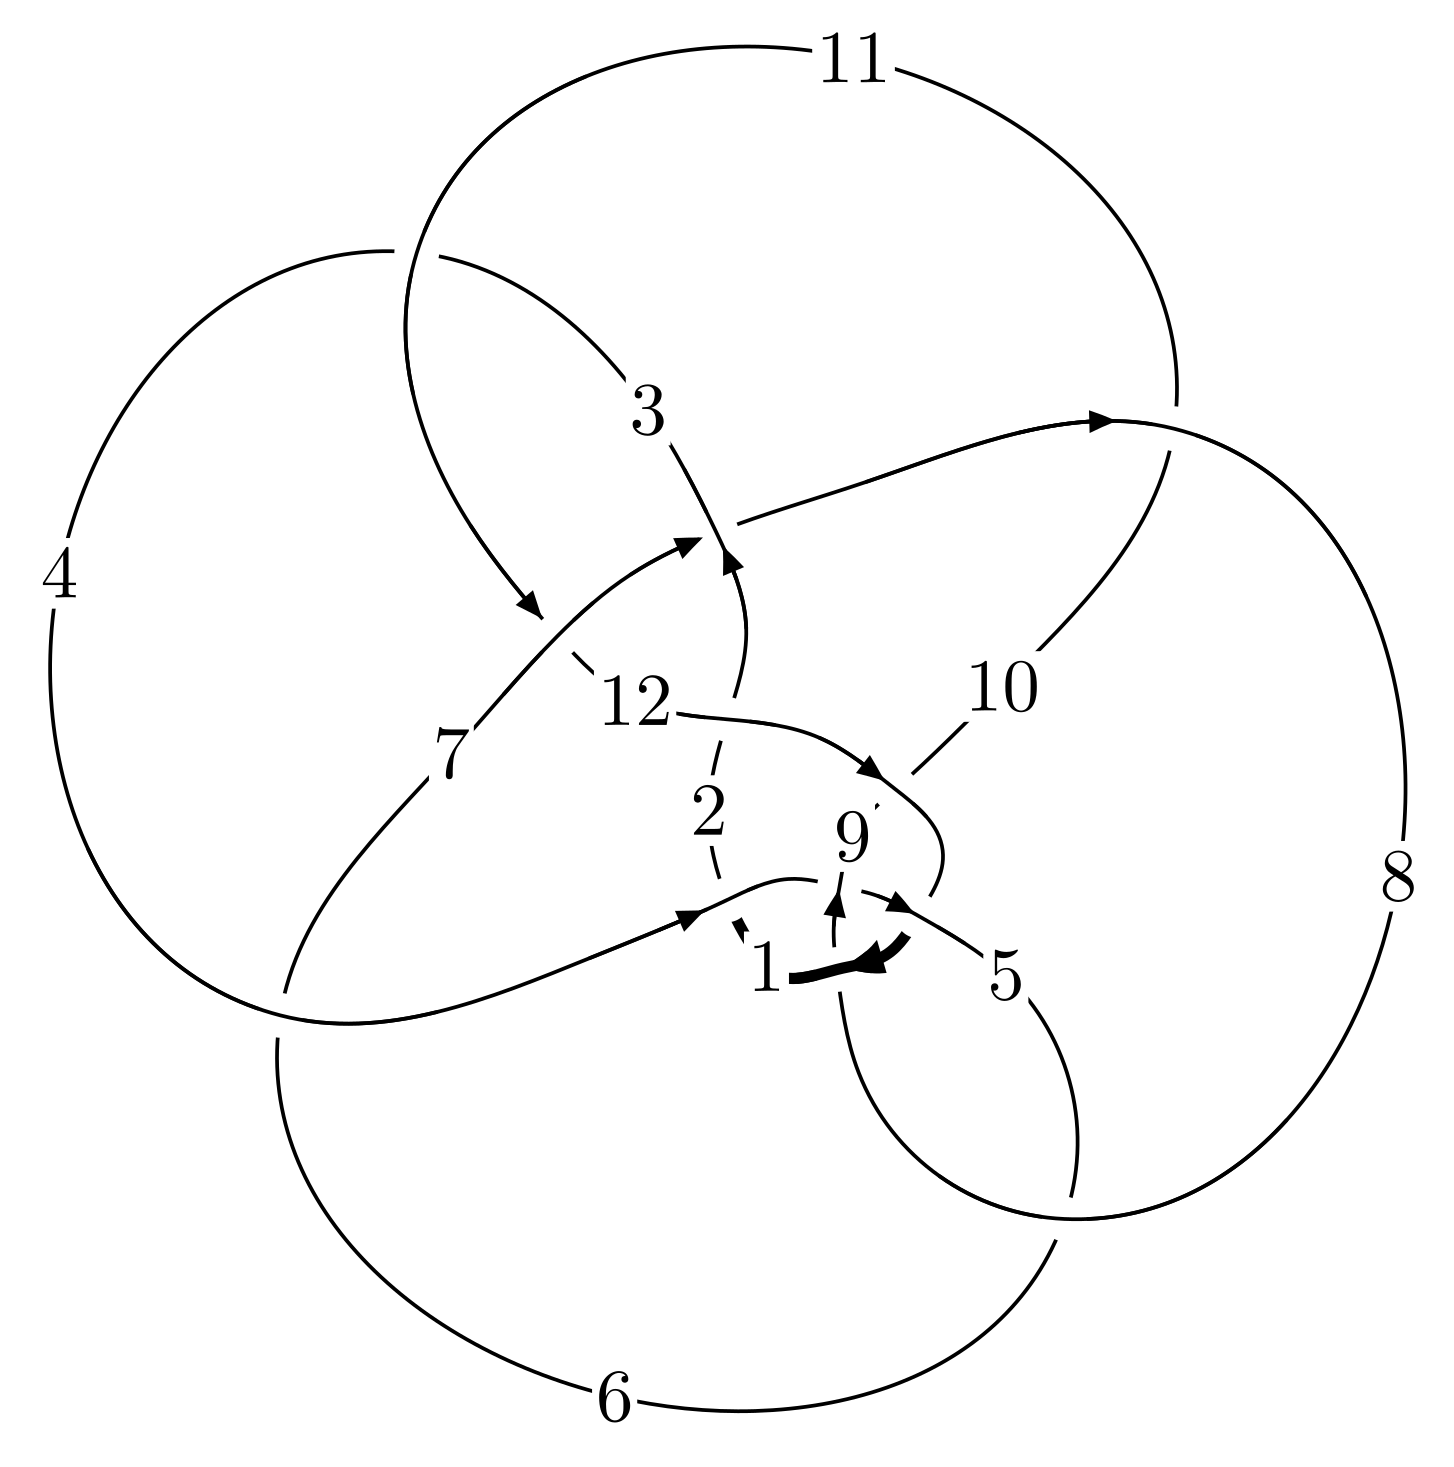
\includegraphics[width=112pt]{../../../GIT/diagram.site/Diagrams/png/2926_12n_0837.png}\\
\ \ \ A knot diagram\footnotemark}&
\allowdisplaybreaks
\textbf{Linearized knot diagam} \\
\cline{2-2}
 &
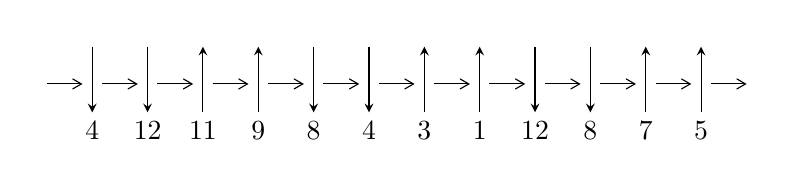
\begin{tikzpicture}[x=20pt, y=17pt]
	% nodes
	\node (C0) at (0, 0) {};
	\node (C1) at (1, 0) {};
	\node (C1U) at (1, +1) {};
	\node (C1D) at (1, -1) {4};

	\node (C2) at (2, 0) {};
	\node (C2U) at (2, +1) {};
	\node (C2D) at (2, -1) {12};

	\node (C3) at (3, 0) {};
	\node (C3U) at (3, +1) {};
	\node (C3D) at (3, -1) {11};

	\node (C4) at (4, 0) {};
	\node (C4U) at (4, +1) {};
	\node (C4D) at (4, -1) {9};

	\node (C5) at (5, 0) {};
	\node (C5U) at (5, +1) {};
	\node (C5D) at (5, -1) {8};

	\node (C6) at (6, 0) {};
	\node (C6U) at (6, +1) {};
	\node (C6D) at (6, -1) {4};

	\node (C7) at (7, 0) {};
	\node (C7U) at (7, +1) {};
	\node (C7D) at (7, -1) {3};

	\node (C8) at (8, 0) {};
	\node (C8U) at (8, +1) {};
	\node (C8D) at (8, -1) {1};

	\node (C9) at (9, 0) {};
	\node (C9U) at (9, +1) {};
	\node (C9D) at (9, -1) {12};

	\node (C10) at (10, 0) {};
	\node (C10U) at (10, +1) {};
	\node (C10D) at (10, -1) {8};

	\node (C11) at (11, 0) {};
	\node (C11U) at (11, +1) {};
	\node (C11D) at (11, -1) {7};

	\node (C12) at (12, 0) {};
	\node (C12U) at (12, +1) {};
	\node (C12D) at (12, -1) {5};
	\node (C13) at (13, 0) {};

	% arrows
	\draw[->,>={angle 60}]
	(C0) edge (C1) (C1) edge (C2) (C2) edge (C3) (C3) edge (C4) (C4) edge (C5) (C5) edge (C6) (C6) edge (C7) (C7) edge (C8) (C8) edge (C9) (C9) edge (C10) (C10) edge (C11) (C11) edge (C12) (C12) edge (C13) ;	\draw[->,>=stealth]
	(C1U) edge (C1D) (C2U) edge (C2D) (C3D) edge (C3U) (C4D) edge (C4U) (C5U) edge (C5D) (C6U) edge (C6D) (C7D) edge (C7U) (C8D) edge (C8U) (C9U) edge (C9D) (C10U) edge (C10D) (C11D) edge (C11U) (C12D) edge (C12U) ;
	\end{tikzpicture} \\
\hhline{~~} \\& 
\textbf{Solving Sequence} \\ \cline{2-2} 
 &
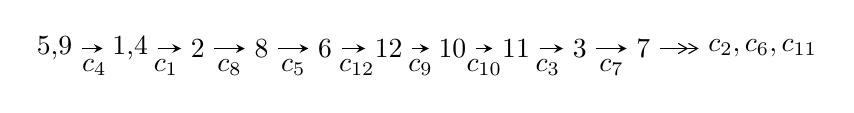
\begin{tikzpicture}[x=23pt, y=7pt]
	% node
	\node (A0) at (-1/8, 0) {5,9};
	\node (A1) at (17/16, 0) {1,4};
	\node (A2) at (17/8, 0) {2};
	\node (A3) at (25/8, 0) {8};
	\node (A4) at (33/8, 0) {6};
	\node (A5) at (41/8, 0) {12};
	\node (A6) at (49/8, 0) {10};
	\node (A7) at (57/8, 0) {11};
	\node (A8) at (65/8, 0) {3};
	\node (A9) at (73/8, 0) {7};
	\node (C1) at (1/2, -1) {$c_{4}$};
	\node (C2) at (13/8, -1) {$c_{1}$};
	\node (C3) at (21/8, -1) {$c_{8}$};
	\node (C4) at (29/8, -1) {$c_{5}$};
	\node (C5) at (37/8, -1) {$c_{12}$};
	\node (C6) at (45/8, -1) {$c_{9}$};
	\node (C7) at (53/8, -1) {$c_{10}$};
	\node (C8) at (61/8, -1) {$c_{3}$};
	\node (C9) at (69/8, -1) {$c_{7}$};
	\node (A10) at (11, 0) {$c_{2},c_{6},c_{11}$};

	% edge
	\draw[->,>=stealth]	
	(A0) edge (A1) (A1) edge (A2) (A2) edge (A3) (A3) edge (A4) (A4) edge (A5) (A5) edge (A6) (A6) edge (A7) (A7) edge (A8) (A8) edge (A9) ;
	\draw[->>,>={angle 60}]	
	(A9) edge (A10);
\end{tikzpicture} \\ 

\end{tabular} \\

\footnotetext{
The image of knot diagram is generated by the software ``\textbf{Draw programme}" developed by Andrew Bartholomew(\url{http://www.layer8.co.uk/maths/draw/index.htm\#Running-draw}), where we modified some parts for our purpose(\url{https://github.com/CATsTAILs/LinksPainter}).
}\phantom \\ \newline 
\centering \textbf{Ideals for irreducible components\footnotemark of $X_{\text{par}}$} 
 
\begin{align*}
I^u_{1}&=\langle 
b+u,\;a-1,\;u^4+2 u^3+2 u^2- u-1\rangle \\
I^u_{2}&=\langle 
b+u,\;-9 u^{17}+40 u^{16}+\cdots+2 a+19,\;u^{18}-5 u^{17}+\cdots-6 u+2\rangle \\
I^u_{3}&=\langle 
5 u^{17}-24 u^{16}+\cdots+2 b-18,\;a-1,\;u^{18}-5 u^{17}+\cdots-6 u+2\rangle \\
I^u_{4}&=\langle 
-1573066898 u^{17}-28039813504 u^{16}+\cdots+6554007584 b-87714720832,\\
\phantom{I^u_{4}}&\phantom{= \langle  }-2741085026 u^{17}-47766463570 u^{16}+\cdots+6554007584 a-96897616096,\\
\phantom{I^u_{4}}&\phantom{= \langle  }2 u^{18}+36 u^{17}+\cdots+288 u+64\rangle \\
I^u_{5}&=\langle 
b+u,\;a+1,\;u^6- u^5+u^4+2 u^3+u+1\rangle \\
I^u_{6}&=\langle 
b+u,\;a+1,\;u^4-2 u^3+2 u^2- u+1\rangle \\
I^u_{7}&=\langle 
u^5- u^4+3 u^3- a u-2 u^2+b+u,\;- u^4 a+u^5+u^3 a- u^4-3 u^2 a+3 u^3+a^2+2 a u-3 u^2- a+2 u-3,\\
\phantom{I^u_{7}}&\phantom{= \langle  }u^6- u^5+3 u^4-2 u^3+2 u^2- u+1\rangle \\
I^u_{8}&=\langle 
-8 u^{11}+27 u^{10}-39 u^9+7 u^8+13 u^7+57 u^6-222 u^5+307 u^4-266 u^3+151 u^2+2 b-61 u+14,\\
\phantom{I^u_{8}}&\phantom{= \langle  }-6 u^{11}+17 u^{10}-19 u^9-7 u^8+7 u^7+49 u^6-138 u^5+147 u^4-106 u^3+47 u^2+2 a-11 u,\\
\phantom{I^u_{8}}&\phantom{= \langle  }u^{12}-4 u^{11}+7 u^{10}-4 u^9- u^8-6 u^7+32 u^6-56 u^5+58 u^4-40 u^3+19 u^2-6 u+1\rangle \\
I^u_{9}&=\langle 
7 u^{11}-23 u^{10}+31 u^9- u^8-13 u^7-54 u^6+189 u^5-242 u^4+193 u^3-103 u^2+2 b+36 u-6,\\
\phantom{I^u_{9}}&\phantom{= \langle  }14 u^{11}-48 u^{10}+71 u^9-17 u^8-21 u^7-97 u^6+391 u^5-562 u^4+505 u^3-294 u^2+2 a+115 u-23,\\
\phantom{I^u_{9}}&\phantom{= \langle  }u^{12}-4 u^{11}+7 u^{10}-4 u^9- u^8-6 u^7+32 u^6-56 u^5+58 u^4-40 u^3+19 u^2-6 u+1\rangle \\
I^u_{10}&=\langle 
b-2 u,\;a-2,\;2 u^2-2 u+1\rangle \\
\end{align*}\\
\begin{align*}
I^u_{11}&=\langle 
b+u,\;2 a-1,\;u^2+2 u+2\rangle \\
I^u_{12}&=\langle 
2 b- u,\;a+1,\;u^2+2 u+2\rangle \\
I^u_{13}&=\langle 
b+u,\;a-1,\;u^6+3 u^5+5 u^4+4 u^3+2 u^2+u+1\rangle \\
I^u_{14}&=\langle 
- u^4+3 u^3- a u-4 u^2+b+u,\;- u^5+u^3 a+2 u^4-3 u^2 a- u^3+a^2+4 a u-4 u^2- a+4 u-4,\\
\phantom{I^u_{14}}&\phantom{= \langle  }u^6-3 u^5+5 u^4-4 u^3+4 u^2- u+1\rangle \\
I^u_{15}&=\langle 
b+u,\;- u^3- u^2+a-1,\;u^4+u^3+u^2+u+1\rangle \\
I^u_{16}&=\langle 
u^2+b+1,\;a+1,\;u^4+u^3+u^2+u+1\rangle \\
I^u_{17}&=\langle 
u^3-3 u^2+b+3 u-1,\;u^3-2 u^2+a+u+1,\;u^4-3 u^3+4 u^2-2 u+1\rangle \\
\\
\end{align*}
\raggedright * 17 irreducible components of $\dim_{\mathbb{C}}=0$, with total 140 representations.\\
\footnotetext{All coefficients of polynomials are rational numbers. But the coefficients are sometimes approximated in decimal forms when there is not enough margin.}
\newpage
\renewcommand{\arraystretch}{1}
\centering \section*{I. $I^u_{1}= \langle b+u,\;a-1,\;u^4+2 u^3+2 u^2- u-1 \rangle$}
\flushleft \textbf{(i) Arc colorings}\\
\begin{tabular}{m{7pt} m{180pt} m{7pt} m{180pt} }
\flushright $a_{5}=$&$\begin{pmatrix}1\\0\end{pmatrix}$ \\
\flushright $a_{9}=$&$\begin{pmatrix}0\\u\end{pmatrix}$ \\
\flushright $a_{1}=$&$\begin{pmatrix}1\\- u\end{pmatrix}$ \\
\flushright $a_{4}=$&$\begin{pmatrix}1\\u^2\end{pmatrix}$ \\
\flushright $a_{2}=$&$\begin{pmatrix}u^2+u+1\\- u^3-2 u^2+1\end{pmatrix}$ \\
\flushright $a_{8}=$&$\begin{pmatrix}- u\\u^2+u\end{pmatrix}$ \\
\flushright $a_{6}=$&$\begin{pmatrix}- u^3- u^2+1\\- u^2+u+1\end{pmatrix}$ \\
\flushright $a_{12}=$&$\begin{pmatrix}u+1\\- u\end{pmatrix}$ \\
\flushright $a_{10}=$&$\begin{pmatrix}- u^3-2 u^2- u\\u^3+u^2+u\end{pmatrix}$ \\
\flushright $a_{11}=$&$\begin{pmatrix}- u^2- u\\u^3+2 u^2-1\end{pmatrix}$ \\
\flushright $a_{3}=$&$\begin{pmatrix}- u^3- u^2+1\\- u^2+1\end{pmatrix}$ \\
\flushright $a_{7}=$&$\begin{pmatrix}- u^3-2 u^2- u+1\\u^3+u^2\end{pmatrix}$\\&\end{tabular}
\flushleft \textbf{(ii) Obstruction class $= -1$}\\~\\
\flushleft \textbf{(iii) Cusp Shapes $= -6 u^3-12 u^2-6 u+9$}\\~\\
\newpage\renewcommand{\arraystretch}{1}
\flushleft \textbf{(iv) u-Polynomials at the component}\newline \\
\begin{tabular}{m{50pt}|m{274pt}}
Crossings & \hspace{64pt}u-Polynomials at each crossing \\
\hline $$\begin{aligned}c_{1},c_{2},c_{5}\\c_{6},c_{9},c_{10}\end{aligned}$$&$\begin{aligned}
&u^4-2 u^3+u^2+4 u-1
\end{aligned}$\\
\hline $$\begin{aligned}c_{3},c_{4},c_{7}\\c_{8},c_{11},c_{12}\end{aligned}$$&$\begin{aligned}
&u^4-2 u^3+2 u^2+u-1
\end{aligned}$\\
\hline
\end{tabular}\\~\\
\newpage\renewcommand{\arraystretch}{1}
\flushleft \textbf{(v) Riley Polynomials at the component}\newline \\
\begin{tabular}{m{50pt}|m{274pt}}
Crossings & \hspace{64pt}Riley Polynomials at each crossing \\
\hline $$\begin{aligned}c_{1},c_{2},c_{5}\\c_{6},c_{9},c_{10}\end{aligned}$$&$\begin{aligned}
&y^4-2 y^3+15 y^2-18 y+1
\end{aligned}$\\
\hline $$\begin{aligned}c_{3},c_{4},c_{7}\\c_{8},c_{11},c_{12}\end{aligned}$$&$\begin{aligned}
&y^4+6 y^2-5 y+1
\end{aligned}$\\
\hline
\end{tabular}\\~\\
\newpage\flushleft \textbf{(vi) Complex Volumes and Cusp Shapes}
$$\begin{array}{c|c|c}  
\text{Solutions to }I^u_{1}& \I (\text{vol} + \sqrt{-1}CS) & \text{Cusp shape}\\
 \hline 
\begin{aligned}
u &= \phantom{-}0.664422\phantom{ +0.000000I} \\
a &= \phantom{-}1.00000\phantom{ +0.000000I} \\
b &= -0.664422\phantom{ +0.000000I}\end{aligned}
 & -2.90924\phantom{ +0.000000I} & -2.04390\phantom{ +0.000000I} \\ \hline\begin{aligned}
u &= -0.591616\phantom{ +0.000000I} \\
a &= \phantom{-}1.00000\phantom{ +0.000000I} \\
b &= \phantom{-}0.591616\phantom{ +0.000000I}\end{aligned}
 & \phantom{-}1.01979\phantom{ +0.000000I} & \phantom{-}9.59200\phantom{ +0.000000I} \\ \hline\begin{aligned}
u &= -1.03640 + 1.21238 I \\
a &= \phantom{-}1.00000\phantom{ +0.000000I} \\
b &= \phantom{-}1.03640 - 1.21238 I\end{aligned}
 & -5.6350 - 19.7459 I & -0.77406 + 10.13367 I \\ \hline\begin{aligned}
u &= -1.03640 - 1.21238 I \\
a &= \phantom{-}1.00000\phantom{ +0.000000I} \\
b &= \phantom{-}1.03640 + 1.21238 I\end{aligned}
 & -5.6350 + 19.7459 I & -0.77406 - 10.13367 I\\
 \hline 
 \end{array}$$\newpage\newpage\renewcommand{\arraystretch}{1}
\centering \section*{II. $I^u_{2}= \langle b+u,\;-9 u^{17}+40 u^{16}+\cdots+2 a+19,\;u^{18}-5 u^{17}+\cdots-6 u+2 \rangle$}
\flushleft \textbf{(i) Arc colorings}\\
\begin{tabular}{m{7pt} m{180pt} m{7pt} m{180pt} }
\flushright $a_{5}=$&$\begin{pmatrix}1\\0\end{pmatrix}$ \\
\flushright $a_{9}=$&$\begin{pmatrix}0\\u\end{pmatrix}$ \\
\flushright $a_{1}=$&$\begin{pmatrix}\frac{9}{2} u^{17}-20 u^{16}+\cdots+\frac{59}{2} u-\frac{19}{2}\\- u\end{pmatrix}$ \\
\flushright $a_{4}=$&$\begin{pmatrix}1\\u^2\end{pmatrix}$ \\
\flushright $a_{2}=$&$\begin{pmatrix}5 u^{17}-\frac{47}{2} u^{16}+\cdots+\frac{73}{2} u-\frac{29}{2}\\-\frac{3}{2} u^{17}+\frac{13}{2} u^{16}+\cdots-8 u+2\end{pmatrix}$ \\
\flushright $a_{8}=$&$\begin{pmatrix}10.2500 u^{17}-44.7500 u^{16}+\cdots+59.2500 u-15.5000\\\frac{1}{2} u^{17}-\frac{7}{2} u^{16}+\cdots+7 u-5\end{pmatrix}$ \\
\flushright $a_{6}=$&$\begin{pmatrix}-\frac{15}{4} u^{17}+\frac{67}{4} u^{16}+\cdots-\frac{77}{4} u+\frac{7}{2}\\u^{17}-4 u^{16}+\cdots-\frac{11}{2} u^2+3 u\end{pmatrix}$ \\
\flushright $a_{12}=$&$\begin{pmatrix}\frac{9}{2} u^{17}-20 u^{16}+\cdots+\frac{61}{2} u-\frac{19}{2}\\- u\end{pmatrix}$ \\
\flushright $a_{10}=$&$\begin{pmatrix}9.25000 u^{17}-37.7500 u^{16}+\cdots+47.2500 u-5.50000\\\frac{1}{2} u^{17}-\frac{7}{2} u^{16}+\cdots+7 u-5\end{pmatrix}$ \\
\flushright $a_{11}=$&$\begin{pmatrix}4 u^{17}-\frac{49}{2} u^{16}+\cdots+\frac{99}{2} u-26\\-\frac{7}{2} u^{17}+15 u^{16}+\cdots-16 u+4\end{pmatrix}$ \\
\flushright $a_{3}=$&$\begin{pmatrix}\frac{1}{2} u^{17}-\frac{13}{2} u^{16}+\cdots+19 u-16\\-\frac{1}{2} u^{17}+\frac{5}{2} u^{16}+\cdots-5 u+2\end{pmatrix}$ \\
\flushright $a_{7}=$&$\begin{pmatrix}-4.75000 u^{17}+21.7500 u^{16}+\cdots-26.7500 u+7.50000\\2 u^{17}-\frac{15}{2} u^{16}+\cdots-\frac{15}{2} u^2+5 u\end{pmatrix}$\\&\end{tabular}
\flushleft \textbf{(ii) Obstruction class $= -1$}\\~\\
\flushleft \textbf{(iii) Cusp Shapes $= -13 u^{17}+63 u^{16}-165 u^{15}+258 u^{14}-297 u^{13}+308 u^{12}-454 u^{11}+751 u^{10}-1156 u^9+1416 u^8-1411 u^7+1045 u^6-635 u^5+324 u^4-212 u^3+137 u^2-92 u+24$}\\~\\
\newpage\renewcommand{\arraystretch}{1}
\flushleft \textbf{(iv) u-Polynomials at the component}\newline \\
\begin{tabular}{m{50pt}|m{274pt}}
Crossings & \hspace{64pt}u-Polynomials at each crossing \\
\hline $$\begin{aligned}c_{1},c_{2},c_{5}\\c_{10}\end{aligned}$$&$\begin{aligned}
&u^{18}+5 u^{17}+\cdots+29 u+11
\end{aligned}$\\
\hline $$\begin{aligned}c_{3},c_{4},c_{11}\\c_{12}\end{aligned}$$&$\begin{aligned}
&u^{18}+5 u^{17}+\cdots+6 u+2
\end{aligned}$\\
\hline $$\begin{aligned}c_{6},c_{9}\end{aligned}$$&$\begin{aligned}
&2(2 u^{18}-42 u^{17}+\cdots-32768 u+4096)
\end{aligned}$\\
\hline $$\begin{aligned}c_{7},c_{8}\end{aligned}$$&$\begin{aligned}
&2(2 u^{18}-36 u^{17}+\cdots-288 u+64)
\end{aligned}$\\
\hline
\end{tabular}\\~\\
\newpage\renewcommand{\arraystretch}{1}
\flushleft \textbf{(v) Riley Polynomials at the component}\newline \\
\begin{tabular}{m{50pt}|m{274pt}}
Crossings & \hspace{64pt}Riley Polynomials at each crossing \\
\hline $$\begin{aligned}c_{1},c_{2},c_{5}\\c_{10}\end{aligned}$$&$\begin{aligned}
&y^{18}-7 y^{17}+\cdots-1171 y+121
\end{aligned}$\\
\hline $$\begin{aligned}c_{3},c_{4},c_{11}\\c_{12}\end{aligned}$$&$\begin{aligned}
&y^{18}+3 y^{17}+\cdots+16 y+4
\end{aligned}$\\
\hline $$\begin{aligned}c_{6},c_{9}\end{aligned}$$&$\begin{aligned}
&4(4 y^{18}-48 y^{17}+\cdots+5242880 y^{2}+1.67772\times10^{7})
\end{aligned}$\\
\hline $$\begin{aligned}c_{7},c_{8}\end{aligned}$$&$\begin{aligned}
&4(4 y^{18}-36 y^{17}+\cdots-50176 y+4096)
\end{aligned}$\\
\hline
\end{tabular}\\~\\
\newpage\flushleft \textbf{(vi) Complex Volumes and Cusp Shapes}
$$\begin{array}{c|c|c}  
\text{Solutions to }I^u_{2}& \I (\text{vol} + \sqrt{-1}CS) & \text{Cusp shape}\\
 \hline 
\begin{aligned}
u &= -0.117461 + 1.055770 I \\
a &= -0.197487 - 0.226554 I \\
b &= \phantom{-}0.117461 - 1.055770 I\end{aligned}
 & -0.27448 - 4.94689 I & -1.21757 + 8.17867 I \\ \hline\begin{aligned}
u &= -0.117461 - 1.055770 I \\
a &= -0.197487 + 0.226554 I \\
b &= \phantom{-}0.117461 + 1.055770 I\end{aligned}
 & -0.27448 + 4.94689 I & -1.21757 - 8.17867 I \\ \hline\begin{aligned}
u &= \phantom{-}0.685691 + 0.586681 I \\
a &= -1.71323 - 0.43588 I \\
b &= -0.685691 - 0.586681 I\end{aligned}
 & -0.27448 + 4.94689 I & -1.21757 - 8.17867 I \\ \hline\begin{aligned}
u &= \phantom{-}0.685691 - 0.586681 I \\
a &= -1.71323 + 0.43588 I \\
b &= -0.685691 + 0.586681 I\end{aligned}
 & -0.27448 - 4.94689 I & -1.21757 + 8.17867 I \\ \hline\begin{aligned}
u &= \phantom{-}0.138696 + 0.833961 I \\
a &= \phantom{-}0.96269 + 1.98234 I \\
b &= -0.138696 - 0.833961 I\end{aligned}
 & -5.85311 - 8.22123 I & -7.71204 + 4.47530 I \\ \hline\begin{aligned}
u &= \phantom{-}0.138696 - 0.833961 I \\
a &= \phantom{-}0.96269 - 1.98234 I \\
b &= -0.138696 + 0.833961 I\end{aligned}
 & -5.85311 + 8.22123 I & -7.71204 - 4.47530 I \\ \hline\begin{aligned}
u &= \phantom{-}0.944753 + 0.780899 I \\
a &= -0.410800 + 0.178193 I \\
b &= -0.944753 - 0.780899 I\end{aligned}
 & \phantom{-}3.08112 - 1.34368 I & \phantom{-}2.02039 + 5.00957 I \\ \hline\begin{aligned}
u &= \phantom{-}0.944753 - 0.780899 I \\
a &= -0.410800 - 0.178193 I \\
b &= -0.944753 + 0.780899 I\end{aligned}
 & \phantom{-}3.08112 + 1.34368 I & \phantom{-}2.02039 - 5.00957 I \\ \hline\begin{aligned}
u &= \phantom{-}0.474610 + 0.583553 I \\
a &= -0.06054 + 2.66696 I \\
b &= -0.474610 - 0.583553 I\end{aligned}
 & -4.67654 + 10.79130 I & -3.31192 - 12.75342 I \\ \hline\begin{aligned}
u &= \phantom{-}0.474610 - 0.583553 I \\
a &= -0.06054 - 2.66696 I \\
b &= -0.474610 + 0.583553 I\end{aligned}
 & -4.67654 - 10.79130 I & -3.31192 + 12.75342 I\\
 \hline 
 \end{array}$$\newpage$$\begin{array}{c|c|c}  
\text{Solutions to }I^u_{2}& \I (\text{vol} + \sqrt{-1}CS) & \text{Cusp shape}\\
 \hline 
\begin{aligned}
u &= -1.105760 + 0.758854 I \\
a &= \phantom{-}0.702132 - 0.134728 I \\
b &= \phantom{-}1.105760 - 0.758854 I\end{aligned}
 & \phantom{-}3.08112 - 1.34368 I & \phantom{-}2.02039 + 5.00957 I \\ \hline\begin{aligned}
u &= -1.105760 - 0.758854 I \\
a &= \phantom{-}0.702132 + 0.134728 I \\
b &= \phantom{-}1.105760 + 0.758854 I\end{aligned}
 & \phantom{-}3.08112 + 1.34368 I & \phantom{-}2.02039 - 5.00957 I \\ \hline\begin{aligned}
u &= -0.462479 + 0.431703 I \\
a &= \phantom{-}1.79515 + 3.21804 I \\
b &= \phantom{-}0.462479 - 0.431703 I\end{aligned}
 & -2.64827\phantom{ +0.000000I} &                  -6
-0.557711 + 0. 10   I\phantom{ +0.000000I} \\ \hline\begin{aligned}
u &= -0.462479 - 0.431703 I \\
a &= \phantom{-}1.79515 - 3.21804 I \\
b &= \phantom{-}0.462479 + 0.431703 I\end{aligned}
 & -2.64827\phantom{ +0.000000I} &                  -6
-0.557711 + 0. 10   I\phantom{ +0.000000I} \\ \hline\begin{aligned}
u &= \phantom{-}0.97105 + 1.12180 I \\
a &= -1.125730 - 0.023180 I \\
b &= -0.97105 - 1.12180 I\end{aligned}
 & -4.67654 + 10.79130 I & -3.31192 - 12.75342 I \\ \hline\begin{aligned}
u &= \phantom{-}0.97105 - 1.12180 I \\
a &= -1.125730 + 0.023180 I \\
b &= -0.97105 + 1.12180 I\end{aligned}
 & -4.67654 - 10.79130 I & -3.31192 + 12.75342 I \\ \hline\begin{aligned}
u &= \phantom{-}0.97090 + 1.14798 I \\
a &= -0.952181 - 0.151413 I \\
b &= -0.97090 - 1.14798 I\end{aligned}
 & -5.85311 + 8.22123 I & -7.71204 - 4.47530 I \\ \hline\begin{aligned}
u &= \phantom{-}0.97090 - 1.14798 I \\
a &= -0.952181 + 0.151413 I \\
b &= -0.97090 + 1.14798 I\end{aligned}
 & -5.85311 - 8.22123 I & -7.71204 + 4.47530 I\\
 \hline 
 \end{array}$$\newpage\newpage\renewcommand{\arraystretch}{1}
\centering \section*{III. $I^u_{3}= \langle 5 u^{17}-24 u^{16}+\cdots+2 b-18,\;a-1,\;u^{18}-5 u^{17}+\cdots-6 u+2 \rangle$}
\flushleft \textbf{(i) Arc colorings}\\
\begin{tabular}{m{7pt} m{180pt} m{7pt} m{180pt} }
\flushright $a_{5}=$&$\begin{pmatrix}1\\0\end{pmatrix}$ \\
\flushright $a_{9}=$&$\begin{pmatrix}0\\u\end{pmatrix}$ \\
\flushright $a_{1}=$&$\begin{pmatrix}1\\-\frac{5}{2} u^{17}+12 u^{16}+\cdots-\frac{35}{2} u+9\end{pmatrix}$ \\
\flushright $a_{4}=$&$\begin{pmatrix}1\\u^2\end{pmatrix}$ \\
\flushright $a_{2}=$&$\begin{pmatrix}\frac{5}{2} u^{17}-12 u^{16}+\cdots+\frac{35}{2} u-8\\-\frac{7}{2} u^{17}+\frac{31}{2} u^{16}+\cdots-\frac{39}{2} u+8\end{pmatrix}$ \\
\flushright $a_{8}=$&$\begin{pmatrix}- u\\\frac{1}{2} u^{17}-\frac{7}{2} u^{16}+\cdots+7 u-5\end{pmatrix}$ \\
\flushright $a_{6}=$&$\begin{pmatrix}u^{17}-\frac{7}{2} u^{16}+\cdots+2 u+2\\u^{17}-4 u^{16}+\cdots-\frac{11}{2} u^2+3 u\end{pmatrix}$ \\
\flushright $a_{12}=$&$\begin{pmatrix}\frac{5}{2} u^{17}-12 u^{16}+\cdots+\frac{35}{2} u-8\\-\frac{5}{2} u^{17}+12 u^{16}+\cdots-\frac{35}{2} u+9\end{pmatrix}$ \\
\flushright $a_{10}=$&$\begin{pmatrix}- u^{16}+4 u^{15}+\cdots+\frac{11}{2} u-3\\-\frac{1}{2} u^{17}+\frac{9}{2} u^{16}+\cdots-\frac{23}{2} u+8\end{pmatrix}$ \\
\flushright $a_{11}=$&$\begin{pmatrix}-2 u^{16}+\frac{15}{2} u^{15}+\cdots+\frac{15}{2} u-5\\\frac{3}{2} u^{17}-7 u^{16}+\cdots+7 u-1\end{pmatrix}$ \\
\flushright $a_{3}=$&$\begin{pmatrix}-2 u^{17}+\frac{13}{2} u^{16}+\cdots- u-4\\u^{17}-4 u^{16}+\cdots+3 u+1\end{pmatrix}$ \\
\flushright $a_{7}=$&$\begin{pmatrix}u^{17}-\frac{9}{2} u^{16}+\cdots+6 u-1\\u^{16}-\frac{7}{2} u^{15}+\cdots-3 u+2\end{pmatrix}$\\&\end{tabular}
\flushleft \textbf{(ii) Obstruction class $= -1$}\\~\\
\flushleft \textbf{(iii) Cusp Shapes $= -13 u^{17}+63 u^{16}-165 u^{15}+258 u^{14}-297 u^{13}+308 u^{12}-454 u^{11}+751 u^{10}-1156 u^9+1416 u^8-1411 u^7+1045 u^6-635 u^5+324 u^4-212 u^3+137 u^2-92 u+24$}\\~\\
\newpage\renewcommand{\arraystretch}{1}
\flushleft \textbf{(iv) u-Polynomials at the component}\newline \\
\begin{tabular}{m{50pt}|m{274pt}}
Crossings & \hspace{64pt}u-Polynomials at each crossing \\
\hline $$\begin{aligned}c_{1},c_{10}\end{aligned}$$&$\begin{aligned}
&2(2 u^{18}-42 u^{17}+\cdots-32768 u+4096)
\end{aligned}$\\
\hline $$\begin{aligned}c_{2},c_{5},c_{6}\\c_{9}\end{aligned}$$&$\begin{aligned}
&u^{18}+5 u^{17}+\cdots+29 u+11
\end{aligned}$\\
\hline $$\begin{aligned}c_{3},c_{4},c_{7}\\c_{8}\end{aligned}$$&$\begin{aligned}
&u^{18}+5 u^{17}+\cdots+6 u+2
\end{aligned}$\\
\hline $$\begin{aligned}c_{11},c_{12}\end{aligned}$$&$\begin{aligned}
&2(2 u^{18}-36 u^{17}+\cdots-288 u+64)
\end{aligned}$\\
\hline
\end{tabular}\\~\\
\newpage\renewcommand{\arraystretch}{1}
\flushleft \textbf{(v) Riley Polynomials at the component}\newline \\
\begin{tabular}{m{50pt}|m{274pt}}
Crossings & \hspace{64pt}Riley Polynomials at each crossing \\
\hline $$\begin{aligned}c_{1},c_{10}\end{aligned}$$&$\begin{aligned}
&4(4 y^{18}-48 y^{17}+\cdots+5242880 y^{2}+1.67772\times10^{7})
\end{aligned}$\\
\hline $$\begin{aligned}c_{2},c_{5},c_{6}\\c_{9}\end{aligned}$$&$\begin{aligned}
&y^{18}-7 y^{17}+\cdots-1171 y+121
\end{aligned}$\\
\hline $$\begin{aligned}c_{3},c_{4},c_{7}\\c_{8}\end{aligned}$$&$\begin{aligned}
&y^{18}+3 y^{17}+\cdots+16 y+4
\end{aligned}$\\
\hline $$\begin{aligned}c_{11},c_{12}\end{aligned}$$&$\begin{aligned}
&4(4 y^{18}-36 y^{17}+\cdots-50176 y+4096)
\end{aligned}$\\
\hline
\end{tabular}\\~\\
\newpage\flushleft \textbf{(vi) Complex Volumes and Cusp Shapes}
$$\begin{array}{c|c|c}  
\text{Solutions to }I^u_{3}& \I (\text{vol} + \sqrt{-1}CS) & \text{Cusp shape}\\
 \hline 
\begin{aligned}
u &= -0.117461 + 1.055770 I \\
a &= \phantom{-}1.00000\phantom{ +0.000000I} \\
b &= -0.262386 + 0.181889 I\end{aligned}
 & -0.27448 - 4.94689 I & -1.21757 + 8.17867 I \\ \hline\begin{aligned}
u &= -0.117461 - 1.055770 I \\
a &= \phantom{-}1.00000\phantom{ +0.000000I} \\
b &= -0.262386 - 0.181889 I\end{aligned}
 & -0.27448 + 4.94689 I & -1.21757 - 8.17867 I \\ \hline\begin{aligned}
u &= \phantom{-}0.685691 + 0.586681 I \\
a &= \phantom{-}1.00000\phantom{ +0.000000I} \\
b &= \phantom{-}0.91902 + 1.30400 I\end{aligned}
 & -0.27448 + 4.94689 I & -1.21757 - 8.17867 I \\ \hline\begin{aligned}
u &= \phantom{-}0.685691 - 0.586681 I \\
a &= \phantom{-}1.00000\phantom{ +0.000000I} \\
b &= \phantom{-}0.91902 - 1.30400 I\end{aligned}
 & -0.27448 - 4.94689 I & -1.21757 + 8.17867 I \\ \hline\begin{aligned}
u &= \phantom{-}0.138696 + 0.833961 I \\
a &= \phantom{-}1.00000\phantom{ +0.000000I} \\
b &= \phantom{-}1.51967 - 1.07779 I\end{aligned}
 & -5.85311 - 8.22123 I & -7.71204 + 4.47530 I \\ \hline\begin{aligned}
u &= \phantom{-}0.138696 - 0.833961 I \\
a &= \phantom{-}1.00000\phantom{ +0.000000I} \\
b &= \phantom{-}1.51967 + 1.07779 I\end{aligned}
 & -5.85311 + 8.22123 I & -7.71204 - 4.47530 I \\ \hline\begin{aligned}
u &= \phantom{-}0.944753 + 0.780899 I \\
a &= \phantom{-}1.00000\phantom{ +0.000000I} \\
b &= \phantom{-}0.527255 + 0.152445 I\end{aligned}
 & \phantom{-}3.08112 - 1.34368 I & \phantom{-}2.02039 + 5.00957 I \\ \hline\begin{aligned}
u &= \phantom{-}0.944753 - 0.780899 I \\
a &= \phantom{-}1.00000\phantom{ +0.000000I} \\
b &= \phantom{-}0.527255 - 0.152445 I\end{aligned}
 & \phantom{-}3.08112 + 1.34368 I & \phantom{-}2.02039 - 5.00957 I \\ \hline\begin{aligned}
u &= \phantom{-}0.474610 + 0.583553 I \\
a &= \phantom{-}1.00000\phantom{ +0.000000I} \\
b &= \phantom{-}1.58505 - 1.23044 I\end{aligned}
 & -4.67654 + 10.79130 I & -3.31192 - 12.75342 I \\ \hline\begin{aligned}
u &= \phantom{-}0.474610 - 0.583553 I \\
a &= \phantom{-}1.00000\phantom{ +0.000000I} \\
b &= \phantom{-}1.58505 + 1.23044 I\end{aligned}
 & -4.67654 - 10.79130 I & -3.31192 + 12.75342 I\\
 \hline 
 \end{array}$$\newpage$$\begin{array}{c|c|c}  
\text{Solutions to }I^u_{3}& \I (\text{vol} + \sqrt{-1}CS) & \text{Cusp shape}\\
 \hline 
\begin{aligned}
u &= -1.105760 + 0.758854 I \\
a &= \phantom{-}1.00000\phantom{ +0.000000I} \\
b &= \phantom{-}0.674150 - 0.681792 I\end{aligned}
 & \phantom{-}3.08112 - 1.34368 I & \phantom{-}2.02039 + 5.00957 I \\ \hline\begin{aligned}
u &= -1.105760 - 0.758854 I \\
a &= \phantom{-}1.00000\phantom{ +0.000000I} \\
b &= \phantom{-}0.674150 + 0.681792 I\end{aligned}
 & \phantom{-}3.08112 + 1.34368 I & \phantom{-}2.02039 - 5.00957 I \\ \hline\begin{aligned}
u &= -0.462479 + 0.431703 I \\
a &= \phantom{-}1.00000\phantom{ +0.000000I} \\
b &= \phantom{-}2.21945 + 0.71331 I\end{aligned}
 & -2.64827\phantom{ +0.000000I} &                  -6
-0.557711 + 0. 10   I\phantom{ +0.000000I} \\ \hline\begin{aligned}
u &= -0.462479 - 0.431703 I \\
a &= \phantom{-}1.00000\phantom{ +0.000000I} \\
b &= \phantom{-}2.21945 - 0.71331 I\end{aligned}
 & -2.64827\phantom{ +0.000000I} &                  -6
-0.557711 + 0. 10   I\phantom{ +0.000000I} \\ \hline\begin{aligned}
u &= \phantom{-}0.97105 + 1.12180 I \\
a &= \phantom{-}1.00000\phantom{ +0.000000I} \\
b &= \phantom{-}1.06713 + 1.28535 I\end{aligned}
 & -4.67654 + 10.79130 I & -3.31192 - 12.75342 I \\ \hline\begin{aligned}
u &= \phantom{-}0.97105 - 1.12180 I \\
a &= \phantom{-}1.00000\phantom{ +0.000000I} \\
b &= \phantom{-}1.06713 - 1.28535 I\end{aligned}
 & -4.67654 - 10.79130 I & -3.31192 + 12.75342 I \\ \hline\begin{aligned}
u &= \phantom{-}0.97090 + 1.14798 I \\
a &= \phantom{-}1.00000\phantom{ +0.000000I} \\
b &= \phantom{-}0.75065 + 1.24009 I\end{aligned}
 & -5.85311 + 8.22123 I & -7.71204 - 4.47530 I \\ \hline\begin{aligned}
u &= \phantom{-}0.97090 - 1.14798 I \\
a &= \phantom{-}1.00000\phantom{ +0.000000I} \\
b &= \phantom{-}0.75065 - 1.24009 I\end{aligned}
 & -5.85311 - 8.22123 I & -7.71204 + 4.47530 I\\
 \hline 
 \end{array}$$\newpage\newpage\renewcommand{\arraystretch}{1}
\centering \section*{IV. $I^u_{4}= \langle -1.57\times10^{9} u^{17}-2.80\times10^{10} u^{16}+\cdots+6.55\times10^{9} b-8.77\times10^{10},\;-2.74\times10^{9} u^{17}-4.78\times10^{10} u^{16}+\cdots+6.55\times10^{9} a-9.69\times10^{10},\;2 u^{18}+36 u^{17}+\cdots+288 u+64 \rangle$}
\flushleft \textbf{(i) Arc colorings}\\
\begin{tabular}{m{7pt} m{180pt} m{7pt} m{180pt} }
\flushright $a_{5}=$&$\begin{pmatrix}1\\0\end{pmatrix}$ \\
\flushright $a_{9}=$&$\begin{pmatrix}0\\u\end{pmatrix}$ \\
\flushright $a_{1}=$&$\begin{pmatrix}0.418230 u^{17}+7.28813 u^{16}+\cdots+55.0668 u+14.7845\\0.240016 u^{17}+4.27827 u^{16}+\cdots+45.4407 u+13.3834\end{pmatrix}$ \\
\flushright $a_{4}=$&$\begin{pmatrix}1\\u^2\end{pmatrix}$ \\
\flushright $a_{2}=$&$\begin{pmatrix}0.220233 u^{17}+3.85283 u^{16}+\cdots+30.8051 u+9.08162\\0.279696 u^{17}+4.70292 u^{16}+\cdots+33.2504 u+9.26644\end{pmatrix}$ \\
\flushright $a_{8}=$&$\begin{pmatrix}-0.405049 u^{17}-7.06890 u^{16}+\cdots-66.2576 u-23.6467\\-0.221980 u^{17}-3.87748 u^{16}+\cdots-33.6803 u-12.9616\end{pmatrix}$ \\
\flushright $a_{6}=$&$\begin{pmatrix}-0.0814254 u^{17}-1.40331 u^{16}+\cdots-6.57667 u-8.03340\\0.0558069 u^{17}+1.04276 u^{16}+\cdots+16.3117 u+4.49774\end{pmatrix}$ \\
\flushright $a_{12}=$&$\begin{pmatrix}0.178214 u^{17}+3.00986 u^{16}+\cdots+9.62612 u+1.40111\\0.240016 u^{17}+4.27827 u^{16}+\cdots+45.4407 u+13.3834\end{pmatrix}$ \\
\flushright $a_{10}=$&$\begin{pmatrix}-0.0792438 u^{17}-1.38641 u^{16}+\cdots-15.9005 u-4.82694\\-0.103825 u^{17}-1.80501 u^{16}+\cdots-14.6768 u-5.85821\end{pmatrix}$ \\
\flushright $a_{11}=$&$\begin{pmatrix}-0.669793 u^{17}-11.6921 u^{16}+\cdots-106.612 u-38.3152\\-0.305026 u^{17}-5.38385 u^{16}+\cdots-51.3580 u-20.0086\end{pmatrix}$ \\
\flushright $a_{3}=$&$\begin{pmatrix}0.407230 u^{17}+7.09082 u^{16}+\cdots+65.9981 u+22.7461\\0.463276 u^{17}+7.95175 u^{16}+\cdots+61.0907 u+21.1249\end{pmatrix}$ \\
\flushright $a_{7}=$&$\begin{pmatrix}-0.229775 u^{17}-3.95065 u^{16}+\cdots-29.2608 u-14.5263\\-0.0526146 u^{17}-0.945653 u^{16}+\cdots+3.35320 u+0.563147\end{pmatrix}$\\&\end{tabular}
\flushleft \textbf{(ii) Obstruction class $= -1$}\\~\\
\flushleft \textbf{(iii) Cusp Shapes $= -\frac{867904991}{819250948} u^{17}-\frac{7549831247}{409625474} u^{16}+\cdots-\frac{35978777006}{204812737} u-\frac{12280937430}{204812737}$}\\~\\
\newpage\renewcommand{\arraystretch}{1}
\flushleft \textbf{(iv) u-Polynomials at the component}\newline \\
\begin{tabular}{m{50pt}|m{274pt}}
Crossings & \hspace{64pt}u-Polynomials at each crossing \\
\hline $$\begin{aligned}c_{1},c_{6},c_{9}\\c_{10}\end{aligned}$$&$\begin{aligned}
&u^{18}+5 u^{17}+\cdots+29 u+11
\end{aligned}$\\
\hline $$\begin{aligned}c_{2},c_{5}\end{aligned}$$&$\begin{aligned}
&2(2 u^{18}-42 u^{17}+\cdots-32768 u+4096)
\end{aligned}$\\
\hline $$\begin{aligned}c_{3},c_{4}\end{aligned}$$&$\begin{aligned}
&2(2 u^{18}-36 u^{17}+\cdots-288 u+64)
\end{aligned}$\\
\hline $$\begin{aligned}c_{7},c_{8},c_{11}\\c_{12}\end{aligned}$$&$\begin{aligned}
&u^{18}+5 u^{17}+\cdots+6 u+2
\end{aligned}$\\
\hline
\end{tabular}\\~\\
\newpage\renewcommand{\arraystretch}{1}
\flushleft \textbf{(v) Riley Polynomials at the component}\newline \\
\begin{tabular}{m{50pt}|m{274pt}}
Crossings & \hspace{64pt}Riley Polynomials at each crossing \\
\hline $$\begin{aligned}c_{1},c_{6},c_{9}\\c_{10}\end{aligned}$$&$\begin{aligned}
&y^{18}-7 y^{17}+\cdots-1171 y+121
\end{aligned}$\\
\hline $$\begin{aligned}c_{2},c_{5}\end{aligned}$$&$\begin{aligned}
&4(4 y^{18}-48 y^{17}+\cdots+5242880 y^{2}+1.67772\times10^{7})
\end{aligned}$\\
\hline $$\begin{aligned}c_{3},c_{4}\end{aligned}$$&$\begin{aligned}
&4(4 y^{18}-36 y^{17}+\cdots-50176 y+4096)
\end{aligned}$\\
\hline $$\begin{aligned}c_{7},c_{8},c_{11}\\c_{12}\end{aligned}$$&$\begin{aligned}
&y^{18}+3 y^{17}+\cdots+16 y+4
\end{aligned}$\\
\hline
\end{tabular}\\~\\
\newpage\flushleft \textbf{(vi) Complex Volumes and Cusp Shapes}
$$\begin{array}{c|c|c}  
\text{Solutions to }I^u_{4}& \I (\text{vol} + \sqrt{-1}CS) & \text{Cusp shape}\\
 \hline 
\begin{aligned}
u &= -0.674150 + 0.681792 I \\
a &= \phantom{-}1.373660 + 0.263583 I \\
b &= \phantom{-}1.105760 - 0.758854 I\end{aligned}
 & \phantom{-}3.08112 - 1.34368 I & \phantom{-}2.02039 + 5.00957 I \\ \hline\begin{aligned}
u &= -0.674150 - 0.681792 I \\
a &= \phantom{-}1.373660 - 0.263583 I \\
b &= \phantom{-}1.105760 + 0.758854 I\end{aligned}
 & \phantom{-}3.08112 + 1.34368 I & \phantom{-}2.02039 - 5.00957 I \\ \hline\begin{aligned}
u &= -0.75065 + 1.24009 I \\
a &= -1.024320 - 0.162884 I \\
b &= -0.97090 + 1.14798 I\end{aligned}
 & -5.85311 - 8.22123 I & -7.71204 + 4.47530 I \\ \hline\begin{aligned}
u &= -0.75065 - 1.24009 I \\
a &= -1.024320 + 0.162884 I \\
b &= -0.97090 - 1.14798 I\end{aligned}
 & -5.85311 + 8.22123 I & -7.71204 - 4.47530 I \\ \hline\begin{aligned}
u &= -0.527255 + 0.152445 I \\
a &= -2.04878 + 0.88870 I \\
b &= -0.944753 + 0.780899 I\end{aligned}
 & \phantom{-}3.08112 + 1.34368 I & \phantom{-}2.02039 - 5.00957 I \\ \hline\begin{aligned}
u &= -0.527255 - 0.152445 I \\
a &= -2.04878 - 0.88870 I \\
b &= -0.944753 - 0.780899 I\end{aligned}
 & \phantom{-}3.08112 - 1.34368 I & \phantom{-}2.02039 + 5.00957 I \\ \hline\begin{aligned}
u &= -0.91902 + 1.30400 I \\
a &= -0.548208 - 0.139474 I \\
b &= -0.685691 + 0.586681 I\end{aligned}
 & -0.27448 - 4.94689 I & -1.21757 + 8.17867 I \\ \hline\begin{aligned}
u &= -0.91902 - 1.30400 I \\
a &= -0.548208 + 0.139474 I \\
b &= -0.685691 - 0.586681 I\end{aligned}
 & -0.27448 + 4.94689 I & -1.21757 - 8.17867 I \\ \hline\begin{aligned}
u &= -1.06713 + 1.28535 I \\
a &= -0.887939 - 0.018284 I \\
b &= -0.97105 + 1.12180 I\end{aligned}
 & -4.67654 - 10.79130 I & -3.31192 + 12.75342 I \\ \hline\begin{aligned}
u &= -1.06713 - 1.28535 I \\
a &= -0.887939 + 0.018284 I \\
b &= -0.97105 - 1.12180 I\end{aligned}
 & -4.67654 + 10.79130 I & -3.31192 - 12.75342 I\\
 \hline 
 \end{array}$$\newpage$$\begin{array}{c|c|c}  
\text{Solutions to }I^u_{4}& \I (\text{vol} + \sqrt{-1}CS) & \text{Cusp shape}\\
 \hline 
\begin{aligned}
u &= \phantom{-}0.262386 + 0.181889 I \\
a &= -2.18634 - 2.50813 I \\
b &= \phantom{-}0.117461 + 1.055770 I\end{aligned}
 & -0.27448 + 4.94689 I & -1.21757 - 8.17867 I \\ \hline\begin{aligned}
u &= \phantom{-}0.262386 - 0.181889 I \\
a &= -2.18634 + 2.50813 I \\
b &= \phantom{-}0.117461 - 1.055770 I\end{aligned}
 & -0.27448 - 4.94689 I & -1.21757 + 8.17867 I \\ \hline\begin{aligned}
u &= -1.51967 + 1.07779 I \\
a &= \phantom{-}0.198230 - 0.408188 I \\
b &= -0.138696 - 0.833961 I\end{aligned}
 & -5.85311 - 8.22123 I & -7.71204 + 4.47530 I \\ \hline\begin{aligned}
u &= -1.51967 - 1.07779 I \\
a &= \phantom{-}0.198230 + 0.408188 I \\
b &= -0.138696 + 0.833961 I\end{aligned}
 & -5.85311 + 8.22123 I & -7.71204 - 4.47530 I \\ \hline\begin{aligned}
u &= -1.58505 + 1.23044 I \\
a &= -0.008508 - 0.374766 I \\
b &= -0.474610 - 0.583553 I\end{aligned}
 & -4.67654 + 10.79130 I & -3.31192 - 12.75342 I \\ \hline\begin{aligned}
u &= -1.58505 - 1.23044 I \\
a &= -0.008508 + 0.374766 I \\
b &= -0.474610 + 0.583553 I\end{aligned}
 & -4.67654 - 10.79130 I & -3.31192 + 12.75342 I \\ \hline\begin{aligned}
u &= -2.21945 + 0.71331 I \\
a &= \phantom{-}0.132207 + 0.236998 I \\
b &= \phantom{-}0.462479 + 0.431703 I\end{aligned}
 & -2.64827\phantom{ +0.000000I} & \phantom{-0.000000 } 0 \\ \hline\begin{aligned}
u &= -2.21945 - 0.71331 I \\
a &= \phantom{-}0.132207 - 0.236998 I \\
b &= \phantom{-}0.462479 - 0.431703 I\end{aligned}
 & -2.64827\phantom{ +0.000000I} & \phantom{-0.000000 } 0\\
 \hline 
 \end{array}$$\newpage\newpage\renewcommand{\arraystretch}{1}
\centering \section*{V. $I^u_{5}= \langle b+u,\;a+1,\;u^6- u^5+u^4+2 u^3+u+1 \rangle$}
\flushleft \textbf{(i) Arc colorings}\\
\begin{tabular}{m{7pt} m{180pt} m{7pt} m{180pt} }
\flushright $a_{5}=$&$\begin{pmatrix}1\\0\end{pmatrix}$ \\
\flushright $a_{9}=$&$\begin{pmatrix}0\\u\end{pmatrix}$ \\
\flushright $a_{1}=$&$\begin{pmatrix}-1\\- u\end{pmatrix}$ \\
\flushright $a_{4}=$&$\begin{pmatrix}1\\u^2\end{pmatrix}$ \\
\flushright $a_{2}=$&$\begin{pmatrix}- u^2+u-1\\- u^4+u^3- u\end{pmatrix}$ \\
\flushright $a_{8}=$&$\begin{pmatrix}- u\\- u^2+u\end{pmatrix}$ \\
\flushright $a_{6}=$&$\begin{pmatrix}u^3- u^2+1\\u^4-2 u^3+u^2\end{pmatrix}$ \\
\flushright $a_{12}=$&$\begin{pmatrix}u-1\\- u\end{pmatrix}$ \\
\flushright $a_{10}=$&$\begin{pmatrix}- u^3+2 u^2- u\\u^3- u^2+u\end{pmatrix}$ \\
\flushright $a_{11}=$&$\begin{pmatrix}u^5- u^4+u^3+2 u^2+1\\- u^5+2 u^4-3 u^3-2\end{pmatrix}$ \\
\flushright $a_{3}=$&$\begin{pmatrix}-2 u^5+3 u^4-4 u^3- u^2-2\\u^5-2 u^4+3 u^3+1\end{pmatrix}$ \\
\flushright $a_{7}=$&$\begin{pmatrix}u^5-2 u^4+3 u^3- u^2+1\\1\end{pmatrix}$\\&\end{tabular}
\flushleft \textbf{(ii) Obstruction class $= 1$}\\~\\
\flushleft \textbf{(iii) Cusp Shapes $= -3 u^5+6 u^4-12 u^3+3 u^2-3 u-12$}\\~\\
\newpage\renewcommand{\arraystretch}{1}
\flushleft \textbf{(iv) u-Polynomials at the component}\newline \\
\begin{tabular}{m{50pt}|m{274pt}}
Crossings & \hspace{64pt}u-Polynomials at each crossing \\
\hline $$\begin{aligned}c_{1},c_{5},c_{9}\end{aligned}$$&$\begin{aligned}
&u^6-2 u^5- u^4+7 u^3-2 u^2-7 u+5
\end{aligned}$\\
\hline $$\begin{aligned}c_{2},c_{6},c_{10}\end{aligned}$$&$\begin{aligned}
&u^6+2 u^5- u^4-7 u^3-2 u^2+7 u+5
\end{aligned}$\\
\hline $$\begin{aligned}c_{3},c_{7},c_{11}\end{aligned}$$&$\begin{aligned}
&u^6+u^5+u^4-2 u^3- u+1
\end{aligned}$\\
\hline $$\begin{aligned}c_{4},c_{8},c_{12}\end{aligned}$$&$\begin{aligned}
&u^6- u^5+u^4+2 u^3+u+1
\end{aligned}$\\
\hline
\end{tabular}\\~\\
\newpage\renewcommand{\arraystretch}{1}
\flushleft \textbf{(v) Riley Polynomials at the component}\newline \\
\begin{tabular}{m{50pt}|m{274pt}}
Crossings & \hspace{64pt}Riley Polynomials at each crossing \\
\hline $$\begin{aligned}c_{1},c_{2},c_{5}\\c_{6},c_{9},c_{10}\end{aligned}$$&$\begin{aligned}
&y^6-6 y^5+25 y^4-63 y^3+92 y^2-69 y+25
\end{aligned}$\\
\hline $$\begin{aligned}c_{3},c_{4},c_{7}\\c_{8},c_{11},c_{12}\end{aligned}$$&$\begin{aligned}
&y^6+y^5+5 y^4-2 y^2- y+1
\end{aligned}$\\
\hline
\end{tabular}\\~\\
\newpage\flushleft \textbf{(vi) Complex Volumes and Cusp Shapes}
$$\begin{array}{c|c|c}  
\text{Solutions to }I^u_{5}& \I (\text{vol} + \sqrt{-1}CS) & \text{Cusp shape}\\
 \hline 
\begin{aligned}
u &= \phantom{-}0.284920 + 0.820791 I \\
a &= -1.00000\phantom{ +0.000000I} \\
b &= -0.284920 - 0.820791 I\end{aligned}
 & -3.96484\phantom{ +0.000000I} & -8.68367 + 0. I\phantom{ +0.000000I} \\ \hline\begin{aligned}
u &= \phantom{-}0.284920 - 0.820791 I \\
a &= -1.00000\phantom{ +0.000000I} \\
b &= -0.284920 + 0.820791 I\end{aligned}
 & -3.96484\phantom{ +0.000000I} & -8.68367 + 0. I\phantom{ +0.000000I} \\ \hline\begin{aligned}
u &= -0.747005 + 0.135499 I \\
a &= -1.00000\phantom{ +0.000000I} \\
b &= \phantom{-}0.747005 - 0.135499 I\end{aligned}
 & -4.59731 + 9.42707 I & -1.65816 - 5.60826 I \\ \hline\begin{aligned}
u &= -0.747005 - 0.135499 I \\
a &= -1.00000\phantom{ +0.000000I} \\
b &= \phantom{-}0.747005 + 0.135499 I\end{aligned}
 & -4.59731 - 9.42707 I & -1.65816 + 5.60826 I \\ \hline\begin{aligned}
u &= \phantom{-}0.96209 + 1.17164 I \\
a &= -1.00000\phantom{ +0.000000I} \\
b &= -0.96209 - 1.17164 I\end{aligned}
 & -4.59731 + 9.42707 I & -1.65816 - 5.60826 I \\ \hline\begin{aligned}
u &= \phantom{-}0.96209 - 1.17164 I \\
a &= -1.00000\phantom{ +0.000000I} \\
b &= -0.96209 + 1.17164 I\end{aligned}
 & -4.59731 - 9.42707 I & -1.65816 + 5.60826 I\\
 \hline 
 \end{array}$$\newpage\newpage\renewcommand{\arraystretch}{1}
\centering \section*{VI. $I^u_{6}= \langle b+u,\;a+1,\;u^4-2 u^3+2 u^2- u+1 \rangle$}
\flushleft \textbf{(i) Arc colorings}\\
\begin{tabular}{m{7pt} m{180pt} m{7pt} m{180pt} }
\flushright $a_{5}=$&$\begin{pmatrix}1\\0\end{pmatrix}$ \\
\flushright $a_{9}=$&$\begin{pmatrix}0\\u\end{pmatrix}$ \\
\flushright $a_{1}=$&$\begin{pmatrix}-1\\- u\end{pmatrix}$ \\
\flushright $a_{4}=$&$\begin{pmatrix}1\\u^2\end{pmatrix}$ \\
\flushright $a_{2}=$&$\begin{pmatrix}- u^2+u-1\\- u^3+2 u^2-2 u+1\end{pmatrix}$ \\
\flushright $a_{8}=$&$\begin{pmatrix}- u\\- u^2+u\end{pmatrix}$ \\
\flushright $a_{6}=$&$\begin{pmatrix}u^3- u^2+1\\- u^2+u-1\end{pmatrix}$ \\
\flushright $a_{12}=$&$\begin{pmatrix}u-1\\- u\end{pmatrix}$ \\
\flushright $a_{10}=$&$\begin{pmatrix}- u^3+2 u^2- u\\u^3- u^2+u\end{pmatrix}$ \\
\flushright $a_{11}=$&$\begin{pmatrix}-2 u^3+3 u^2- u\\u^3+1\end{pmatrix}$ \\
\flushright $a_{3}=$&$\begin{pmatrix}u^3-3 u^2+2 u-1\\-2 u^3+3 u^2-2 u+1\end{pmatrix}$ \\
\flushright $a_{7}=$&$\begin{pmatrix}u^3- u+1\\u^3-3 u^2+2 u-2\end{pmatrix}$\\&\end{tabular}
\flushleft \textbf{(ii) Obstruction class $= 1$}\\~\\
\flushleft \textbf{(iii) Cusp Shapes $= -6 u^3+6 u-3$}\\~\\
\newpage\renewcommand{\arraystretch}{1}
\flushleft \textbf{(iv) u-Polynomials at the component}\newline \\
\begin{tabular}{m{50pt}|m{274pt}}
Crossings & \hspace{64pt}u-Polynomials at each crossing \\
\hline $$\begin{aligned}c_{1},c_{5},c_{9}\end{aligned}$$&$\begin{aligned}
&(u^2- u+1)^2
\end{aligned}$\\
\hline $$\begin{aligned}c_{2},c_{6},c_{10}\end{aligned}$$&$\begin{aligned}
&(u^2+u+1)^2
\end{aligned}$\\
\hline $$\begin{aligned}c_{3},c_{7},c_{11}\end{aligned}$$&$\begin{aligned}
&u^4+2 u^3+2 u^2+u+1
\end{aligned}$\\
\hline $$\begin{aligned}c_{4},c_{8},c_{12}\end{aligned}$$&$\begin{aligned}
&u^4-2 u^3+2 u^2- u+1
\end{aligned}$\\
\hline
\end{tabular}\\~\\
\newpage\renewcommand{\arraystretch}{1}
\flushleft \textbf{(v) Riley Polynomials at the component}\newline \\
\begin{tabular}{m{50pt}|m{274pt}}
Crossings & \hspace{64pt}Riley Polynomials at each crossing \\
\hline $$\begin{aligned}c_{1},c_{2},c_{5}\\c_{6},c_{9},c_{10}\end{aligned}$$&$\begin{aligned}
&(y^2+y+1)^2
\end{aligned}$\\
\hline $$\begin{aligned}c_{3},c_{4},c_{7}\\c_{8},c_{11},c_{12}\end{aligned}$$&$\begin{aligned}
&y^4+2 y^2+3 y+1
\end{aligned}$\\
\hline
\end{tabular}\\~\\
\newpage\flushleft \textbf{(vi) Complex Volumes and Cusp Shapes}
$$\begin{array}{c|c|c}  
\text{Solutions to }I^u_{6}& \I (\text{vol} + \sqrt{-1}CS) & \text{Cusp shape}\\
 \hline 
\begin{aligned}
u &= -0.070696 + 0.758745 I \\
a &= -1.00000\phantom{ +0.000000I} \\
b &= \phantom{-}0.070696 - 0.758745 I\end{aligned}
 & -1.74699 - 3.49426 I & -4.15464 + 7.10504 I \\ \hline\begin{aligned}
u &= -0.070696 - 0.758745 I \\
a &= -1.00000\phantom{ +0.000000I} \\
b &= \phantom{-}0.070696 + 0.758745 I\end{aligned}
 & -1.74699 + 3.49426 I & -4.15464 - 7.10504 I \\ \hline\begin{aligned}
u &= \phantom{-}1.070700 + 0.758745 I \\
a &= -1.00000\phantom{ +0.000000I} \\
b &= -1.070700 - 0.758745 I\end{aligned}
 & \phantom{-}5.03685 + 8.68504 I & \phantom{-}7.15464 - 8.48342 I \\ \hline\begin{aligned}
u &= \phantom{-}1.070700 - 0.758745 I \\
a &= -1.00000\phantom{ +0.000000I} \\
b &= -1.070700 + 0.758745 I\end{aligned}
 & \phantom{-}5.03685 - 8.68504 I & \phantom{-}7.15464 + 8.48342 I\\
 \hline 
 \end{array}$$\newpage\newpage\renewcommand{\arraystretch}{1}
\centering \section*{VII. $I^u_{7}= \langle u^5- u^4+3 u^3- a u-2 u^2+b+u,\;- u^4 a+u^5+\cdots- a-3,\;u^6- u^5+3 u^4-2 u^3+2 u^2- u+1 \rangle$}
\flushleft \textbf{(i) Arc colorings}\\
\begin{tabular}{m{7pt} m{180pt} m{7pt} m{180pt} }
\flushright $a_{5}=$&$\begin{pmatrix}1\\0\end{pmatrix}$ \\
\flushright $a_{9}=$&$\begin{pmatrix}0\\u\end{pmatrix}$ \\
\flushright $a_{1}=$&$\begin{pmatrix}a\\- u^5+u^4-3 u^3+a u+2 u^2- u\end{pmatrix}$ \\
\flushright $a_{4}=$&$\begin{pmatrix}1\\u^2\end{pmatrix}$ \\
\flushright $a_{2}=$&$\begin{pmatrix}u^5- u^4+u^2 a+3 u^3- a u-2 u^2+a+u\\u^4 a- u^5- u^3 a+u^4-4 u^3+a u+3 u^2-2 u\end{pmatrix}$ \\
\flushright $a_{8}=$&$\begin{pmatrix}- u^5 a+u^4 a-3 u^3 a+2 u^2 a- u^3- a u-2 u-1\\- u^4-2 u^2\end{pmatrix}$ \\
\flushright $a_{6}=$&$\begin{pmatrix}- u^5 a+u^4 a+2 u^5-3 u^3 a+2 u^2 a+4 u^3-2 a u+u^2\\u^5-2 u^4+3 u^3-4 u^2+u-2\end{pmatrix}$ \\
\flushright $a_{12}=$&$\begin{pmatrix}u^5- u^4+3 u^3- a u-2 u^2+a+u\\- u^5+u^4-3 u^3+a u+2 u^2- u\end{pmatrix}$ \\
\flushright $a_{10}=$&$\begin{pmatrix}- u^5 a+u^4 a-4 u^3 a+u^4+3 u^2 a- u^3-2 a u+3 u^2- u\\u^3 a- u^2 a+a u- u^2+u-1\end{pmatrix}$ \\
\flushright $a_{11}=$&$\begin{pmatrix}- u^5 a+u^5-2 u^3 a- u^4+3 u^3+a u-2 u^2+2 u-2\\u^4 a+u^3 a+u^2 a- u^2+a\end{pmatrix}$ \\
\flushright $a_{3}=$&$\begin{pmatrix}- u^5 a+u^4 a-2 u^3 a+3 u^2 a- a u+a- u\\u^5 a+u^4 a+u^3 a- u^3+a u+u^2\end{pmatrix}$ \\
\flushright $a_{7}=$&$\begin{pmatrix}- u^5 a+u^4 a+u^5-3 u^3 a+u^4+u^2 a+u^3- a u+3 u^2- u\\- u^4 a+u^5+u^3 a-2 u^4+4 u^3-5 u^2+2 u-2\end{pmatrix}$\\&\end{tabular}
\flushleft \textbf{(ii) Obstruction class $= -1$}\\~\\
\flushleft \textbf{(iii) Cusp Shapes $= -8 u^5-20 u^3-8 u^2-6$}\\~\\
\newpage\renewcommand{\arraystretch}{1}
\flushleft \textbf{(iv) u-Polynomials at the component}\newline \\
\begin{tabular}{m{50pt}|m{274pt}}
Crossings & \hspace{64pt}u-Polynomials at each crossing \\
\hline $$\begin{aligned}c_{1},c_{6},c_{9}\\c_{10}\end{aligned}$$&$\begin{aligned}
&u^{12}+4 u^{11}+\cdots+4 u+1
\end{aligned}$\\
\hline $$\begin{aligned}c_{2},c_{5}\end{aligned}$$&$\begin{aligned}
&(u^6+3 u^5+7 u^4+10 u^3+10 u^2+7 u+3)^2
\end{aligned}$\\
\hline $$\begin{aligned}c_{3},c_{4}\end{aligned}$$&$\begin{aligned}
&(u^6+u^5+3 u^4+2 u^3+2 u^2+u+1)^2
\end{aligned}$\\
\hline $$\begin{aligned}c_{7},c_{8},c_{11}\\c_{12}\end{aligned}$$&$\begin{aligned}
&u^{12}+4 u^{11}+\cdots+6 u+1
\end{aligned}$\\
\hline
\end{tabular}\\~\\
\newpage\renewcommand{\arraystretch}{1}
\flushleft \textbf{(v) Riley Polynomials at the component}\newline \\
\begin{tabular}{m{50pt}|m{274pt}}
Crossings & \hspace{64pt}Riley Polynomials at each crossing \\
\hline $$\begin{aligned}c_{1},c_{6},c_{9}\\c_{10}\end{aligned}$$&$\begin{aligned}
&y^{12}-10 y^{11}+\cdots-14 y+1
\end{aligned}$\\
\hline $$\begin{aligned}c_{2},c_{5}\end{aligned}$$&$\begin{aligned}
&(y^6+5 y^5+9 y^4+4 y^3+2 y^2+11 y+9)^2
\end{aligned}$\\
\hline $$\begin{aligned}c_{3},c_{4}\end{aligned}$$&$\begin{aligned}
&(y^6+5 y^5+9 y^4+8 y^3+6 y^2+3 y+1)^2
\end{aligned}$\\
\hline $$\begin{aligned}c_{7},c_{8},c_{11}\\c_{12}\end{aligned}$$&$\begin{aligned}
&y^{12}-2 y^{11}+\cdots+2 y+1
\end{aligned}$\\
\hline
\end{tabular}\\~\\
\newpage\flushleft \textbf{(vi) Complex Volumes and Cusp Shapes}
$$\begin{array}{c|c|c}  
\text{Solutions to }I^u_{7}& \I (\text{vol} + \sqrt{-1}CS) & \text{Cusp shape}\\
 \hline 
\begin{aligned}
u &= \phantom{-}0.616765 + 0.580357 I \\
a &= \phantom{-}1.57092 + 0.24410 I \\
b &= \phantom{-}1.30393 + 0.83343 I\end{aligned}
 & \phantom{-}2.18727 + 7.89459 I & \phantom{-}4.23219 - 13.00098 I \\ \hline\begin{aligned}
u &= \phantom{-}0.616765 + 0.580357 I \\
a &= -1.79571 + 0.33842 I \\
b &= -0.827224 - 1.062250 I\end{aligned}
 & \phantom{-}2.18727 + 7.89459 I & \phantom{-}4.23219 - 13.00098 I \\ \hline\begin{aligned}
u &= \phantom{-}0.616765 - 0.580357 I \\
a &= \phantom{-}1.57092 - 0.24410 I \\
b &= \phantom{-}1.30393 - 0.83343 I\end{aligned}
 & \phantom{-}2.18727 - 7.89459 I & \phantom{-}4.23219 + 13.00098 I \\ \hline\begin{aligned}
u &= \phantom{-}0.616765 - 0.580357 I \\
a &= -1.79571 - 0.33842 I \\
b &= -0.827224 + 1.062250 I\end{aligned}
 & \phantom{-}2.18727 - 7.89459 I & \phantom{-}4.23219 + 13.00098 I \\ \hline\begin{aligned}
u &= -0.291649 + 0.757555 I \\
a &= -0.923318 - 0.267732 I \\
b &= -1.26214 - 1.01347 I\end{aligned}
 & -3.90376 - 2.86500 I & -8.91554 + 9.10702 I \\ \hline\begin{aligned}
u &= -0.291649 + 0.757555 I \\
a &= \phantom{-}0.60651 - 1.89957 I \\
b &= -0.472106 + 0.621380 I\end{aligned}
 & -3.90376 - 2.86500 I & -8.91554 + 9.10702 I \\ \hline\begin{aligned}
u &= -0.291649 - 0.757555 I \\
a &= -0.923318 + 0.267732 I \\
b &= -1.26214 + 1.01347 I\end{aligned}
 & -3.90376 + 2.86500 I & -8.91554 - 9.10702 I \\ \hline\begin{aligned}
u &= -0.291649 - 0.757555 I \\
a &= \phantom{-}0.60651 + 1.89957 I \\
b &= -0.472106 - 0.621380 I\end{aligned}
 & -3.90376 + 2.86500 I & -8.91554 - 9.10702 I \\ \hline\begin{aligned}
u &= \phantom{-}0.17488 + 1.44407 I \\
a &= -0.077332 - 0.438982 I \\
b &= -0.122069 + 0.573149 I\end{aligned}
 & -3.21831 - 0.69024 I & \phantom{-}2.68334 + 10.61298 I \\ \hline\begin{aligned}
u &= \phantom{-}0.17488 + 1.44407 I \\
a &= -0.381072 - 0.130681 I \\
b &= -0.620396 + 0.188443 I\end{aligned}
 & -3.21831 - 0.69024 I & \phantom{-}2.68334 + 10.61298 I\\
 \hline 
 \end{array}$$\newpage$$\begin{array}{c|c|c}  
\text{Solutions to }I^u_{7}& \I (\text{vol} + \sqrt{-1}CS) & \text{Cusp shape}\\
 \hline 
\begin{aligned}
u &= \phantom{-}0.17488 - 1.44407 I \\
a &= -0.077332 + 0.438982 I \\
b &= -0.122069 - 0.573149 I\end{aligned}
 & -3.21831 + 0.69024 I & \phantom{-}2.68334 - 10.61298 I \\ \hline\begin{aligned}
u &= \phantom{-}0.17488 - 1.44407 I \\
a &= -0.381072 + 0.130681 I \\
b &= -0.620396 - 0.188443 I\end{aligned}
 & -3.21831 + 0.69024 I & \phantom{-}2.68334 - 10.61298 I\\
 \hline 
 \end{array}$$\newpage\newpage\renewcommand{\arraystretch}{1}
\centering \section*{VIII. $I^u_{8}= \langle -8 u^{11}+27 u^{10}+\cdots+2 b+14,\;-6 u^{11}+17 u^{10}+\cdots+2 a-11 u,\;u^{12}-4 u^{11}+\cdots-6 u+1 \rangle$}
\flushleft \textbf{(i) Arc colorings}\\
\begin{tabular}{m{7pt} m{180pt} m{7pt} m{180pt} }
\flushright $a_{5}=$&$\begin{pmatrix}1\\0\end{pmatrix}$ \\
\flushright $a_{9}=$&$\begin{pmatrix}0\\u\end{pmatrix}$ \\
\flushright $a_{1}=$&$\begin{pmatrix}3 u^{11}-\frac{17}{2} u^{10}+\cdots-\frac{47}{2} u^2+\frac{11}{2} u\\4 u^{11}-\frac{27}{2} u^{10}+\cdots+\frac{61}{2} u-7\end{pmatrix}$ \\
\flushright $a_{4}=$&$\begin{pmatrix}1\\u^2\end{pmatrix}$ \\
\flushright $a_{2}=$&$\begin{pmatrix}\frac{3}{2} u^{11}-4 u^{10}+\cdots-7 u+\frac{7}{2}\\\frac{5}{2} u^{11}-\frac{17}{2} u^{10}+\cdots+23 u-\frac{11}{2}\end{pmatrix}$ \\
\flushright $a_{8}=$&$\begin{pmatrix}\frac{1}{2} u^{11}-\frac{9}{2} u^{10}+\cdots+16 u-3\\-\frac{5}{2} u^{11}+\frac{19}{2} u^{10}+\cdots-\frac{41}{2} u+5\end{pmatrix}$ \\
\flushright $a_{6}=$&$\begin{pmatrix}-4 u^{11}+16 u^{10}+\cdots-41 u+\frac{19}{2}\\- u^{11}+\frac{9}{2} u^{10}+\cdots-\frac{33}{2} u+5\end{pmatrix}$ \\
\flushright $a_{12}=$&$\begin{pmatrix}- u^{11}+5 u^{10}+\cdots-25 u+7\\4 u^{11}-\frac{27}{2} u^{10}+\cdots+\frac{61}{2} u-7\end{pmatrix}$ \\
\flushright $a_{10}=$&$\begin{pmatrix}6 u^{11}-24 u^{10}+\cdots+56 u-12\\-3 u^{11}+10 u^{10}+\cdots-\frac{35}{2} u+4\end{pmatrix}$ \\
\flushright $a_{11}=$&$\begin{pmatrix}3 u^{11}-11 u^{10}+\cdots+\frac{49}{2} u-6\\3 u^{11}-10 u^{10}+\cdots+21 u-4\end{pmatrix}$ \\
\flushright $a_{3}=$&$\begin{pmatrix}\frac{15}{2} u^{11}-28 u^{10}+\cdots+49 u-\frac{17}{2}\\-\frac{1}{2} u^{11}+\frac{3}{2} u^{10}+\cdots+\frac{9}{2} u-\frac{3}{2}\end{pmatrix}$ \\
\flushright $a_{7}=$&$\begin{pmatrix}-\frac{3}{2} u^{11}+\frac{13}{2} u^{10}+\cdots-\frac{41}{2} u+\frac{9}{2}\\-2 u^{11}+7 u^{10}+\cdots-16 u+\frac{9}{2}\end{pmatrix}$\\&\end{tabular}
\flushleft \textbf{(ii) Obstruction class $= -1$}\\~\\
\flushleft \textbf{(iii) Cusp Shapes $= -42 u^{11}+148 u^{10}-218 u^9+46 u^8+84 u^7+300 u^6-1216 u^5+1720 u^4-1468 u^3+822 u^2-320 u+70$}\\~\\
\newpage\renewcommand{\arraystretch}{1}
\flushleft \textbf{(iv) u-Polynomials at the component}\newline \\
\begin{tabular}{m{50pt}|m{274pt}}
Crossings & \hspace{64pt}u-Polynomials at each crossing \\
\hline $$\begin{aligned}c_{1},c_{10}\end{aligned}$$&$\begin{aligned}
&(u^6+3 u^5+7 u^4+10 u^3+10 u^2+7 u+3)^2
\end{aligned}$\\
\hline $$\begin{aligned}c_{2},c_{5},c_{6}\\c_{9}\end{aligned}$$&$\begin{aligned}
&u^{12}+4 u^{11}+\cdots+4 u+1
\end{aligned}$\\
\hline $$\begin{aligned}c_{3},c_{4},c_{7}\\c_{8}\end{aligned}$$&$\begin{aligned}
&u^{12}+4 u^{11}+\cdots+6 u+1
\end{aligned}$\\
\hline $$\begin{aligned}c_{11},c_{12}\end{aligned}$$&$\begin{aligned}
&(u^6+u^5+3 u^4+2 u^3+2 u^2+u+1)^2
\end{aligned}$\\
\hline
\end{tabular}\\~\\
\newpage\renewcommand{\arraystretch}{1}
\flushleft \textbf{(v) Riley Polynomials at the component}\newline \\
\begin{tabular}{m{50pt}|m{274pt}}
Crossings & \hspace{64pt}Riley Polynomials at each crossing \\
\hline $$\begin{aligned}c_{1},c_{10}\end{aligned}$$&$\begin{aligned}
&(y^6+5 y^5+9 y^4+4 y^3+2 y^2+11 y+9)^2
\end{aligned}$\\
\hline $$\begin{aligned}c_{2},c_{5},c_{6}\\c_{9}\end{aligned}$$&$\begin{aligned}
&y^{12}-10 y^{11}+\cdots-14 y+1
\end{aligned}$\\
\hline $$\begin{aligned}c_{3},c_{4},c_{7}\\c_{8}\end{aligned}$$&$\begin{aligned}
&y^{12}-2 y^{11}+\cdots+2 y+1
\end{aligned}$\\
\hline $$\begin{aligned}c_{11},c_{12}\end{aligned}$$&$\begin{aligned}
&(y^6+5 y^5+9 y^4+8 y^3+6 y^2+3 y+1)^2
\end{aligned}$\\
\hline
\end{tabular}\\~\\
\newpage\flushleft \textbf{(vi) Complex Volumes and Cusp Shapes}
$$\begin{array}{c|c|c}  
\text{Solutions to }I^u_{8}& \I (\text{vol} + \sqrt{-1}CS) & \text{Cusp shape}\\
 \hline 
\begin{aligned}
u &= \phantom{-}0.472106 + 0.621380 I \\
a &= -0.05564 - 2.07346 I \\
b &= \phantom{-}0.291649 + 0.757555 I\end{aligned}
 & -3.90376 + 2.86500 I & -8.91554 - 9.10702 I \\ \hline\begin{aligned}
u &= \phantom{-}0.472106 - 0.621380 I \\
a &= -0.05564 + 2.07346 I \\
b &= \phantom{-}0.291649 - 0.757555 I\end{aligned}
 & -3.90376 - 2.86500 I & -8.91554 + 9.10702 I \\ \hline\begin{aligned}
u &= \phantom{-}0.827224 + 1.062250 I \\
a &= -1.083450 + 0.383784 I \\
b &= -0.616765 - 0.580357 I\end{aligned}
 & \phantom{-}2.18727 + 7.89459 I & \phantom{-}4.23219 - 13.00098 I \\ \hline\begin{aligned}
u &= \phantom{-}0.827224 - 1.062250 I \\
a &= -1.083450 - 0.383784 I \\
b &= -0.616765 + 0.580357 I\end{aligned}
 & \phantom{-}2.18727 - 7.89459 I & \phantom{-}4.23219 + 13.00098 I \\ \hline\begin{aligned}
u &= \phantom{-}0.620396 + 0.188443 I \\
a &= \phantom{-}0.437050 + 0.791090 I \\
b &= -0.17488 + 1.44407 I\end{aligned}
 & -3.21831 + 0.69024 I & \phantom{-}2.68334 - 10.61298 I \\ \hline\begin{aligned}
u &= \phantom{-}0.620396 - 0.188443 I \\
a &= \phantom{-}0.437050 - 0.791090 I \\
b &= -0.17488 - 1.44407 I\end{aligned}
 & -3.21831 - 0.69024 I & \phantom{-}2.68334 + 10.61298 I \\ \hline\begin{aligned}
u &= \phantom{-}0.122069 + 0.573149 I \\
a &= \phantom{-}0.535052 - 0.968480 I \\
b &= -0.17488 + 1.44407 I\end{aligned}
 & -3.21831 + 0.69024 I & \phantom{-}2.68334 - 10.61298 I \\ \hline\begin{aligned}
u &= \phantom{-}0.122069 - 0.573149 I \\
a &= \phantom{-}0.535052 + 0.968480 I \\
b &= -0.17488 - 1.44407 I\end{aligned}
 & -3.21831 - 0.69024 I & \phantom{-}2.68334 + 10.61298 I \\ \hline\begin{aligned}
u &= -1.30393 + 0.83343 I \\
a &= -0.820076 + 0.290489 I \\
b &= -0.616765 + 0.580357 I\end{aligned}
 & \phantom{-}2.18727 - 7.89459 I & \phantom{-}4.23219 + 13.00098 I \\ \hline\begin{aligned}
u &= -1.30393 - 0.83343 I \\
a &= -0.820076 - 0.290489 I \\
b &= -0.616765 - 0.580357 I\end{aligned}
 & \phantom{-}2.18727 + 7.89459 I & \phantom{-}4.23219 - 13.00098 I\\
 \hline 
 \end{array}$$\newpage$$\begin{array}{c|c|c}  
\text{Solutions to }I^u_{8}& \I (\text{vol} + \sqrt{-1}CS) & \text{Cusp shape}\\
 \hline 
\begin{aligned}
u &= \phantom{-}1.26214 + 1.01347 I \\
a &= -0.012932 - 0.481939 I \\
b &= \phantom{-}0.291649 - 0.757555 I\end{aligned}
 & -3.90376 - 2.86500 I & -8.91554 + 9.10702 I \\ \hline\begin{aligned}
u &= \phantom{-}1.26214 - 1.01347 I \\
a &= -0.012932 + 0.481939 I \\
b &= \phantom{-}0.291649 + 0.757555 I\end{aligned}
 & -3.90376 + 2.86500 I & -8.91554 - 9.10702 I\\
 \hline 
 \end{array}$$\newpage\newpage\renewcommand{\arraystretch}{1}
\centering \section*{IX. $I^u_{9}= \langle 7 u^{11}-23 u^{10}+\cdots+2 b-6,\;14 u^{11}-48 u^{10}+\cdots+2 a-23,\;u^{12}-4 u^{11}+\cdots-6 u+1 \rangle$}
\flushleft \textbf{(i) Arc colorings}\\
\begin{tabular}{m{7pt} m{180pt} m{7pt} m{180pt} }
\flushright $a_{5}=$&$\begin{pmatrix}1\\0\end{pmatrix}$ \\
\flushright $a_{9}=$&$\begin{pmatrix}0\\u\end{pmatrix}$ \\
\flushright $a_{1}=$&$\begin{pmatrix}-7 u^{11}+24 u^{10}+\cdots-\frac{115}{2} u+\frac{23}{2}\\-\frac{7}{2} u^{11}+\frac{23}{2} u^{10}+\cdots-18 u+3\end{pmatrix}$ \\
\flushright $a_{4}=$&$\begin{pmatrix}1\\u^2\end{pmatrix}$ \\
\flushright $a_{2}=$&$\begin{pmatrix}-6 u^{11}+21 u^{10}+\cdots-\frac{113}{2} u+\frac{25}{2}\\-\frac{7}{2} u^{11}+\frac{21}{2} u^{10}+\cdots-13 u+2\end{pmatrix}$ \\
\flushright $a_{8}=$&$\begin{pmatrix}-3 u^{11}+11 u^{10}+\cdots-\frac{63}{2} u+10\\-\frac{5}{2} u^{11}+\frac{19}{2} u^{10}+\cdots-\frac{41}{2} u+5\end{pmatrix}$ \\
\flushright $a_{6}=$&$\begin{pmatrix}-5 u^{11}+\frac{37}{2} u^{10}+\cdots-\frac{105}{2} u+\frac{31}{2}\\- u^{11}+\frac{9}{2} u^{10}+\cdots-\frac{33}{2} u+5\end{pmatrix}$ \\
\flushright $a_{12}=$&$\begin{pmatrix}-\frac{7}{2} u^{11}+\frac{25}{2} u^{10}+\cdots-\frac{79}{2} u+\frac{17}{2}\\-\frac{7}{2} u^{11}+\frac{23}{2} u^{10}+\cdots-18 u+3\end{pmatrix}$ \\
\flushright $a_{10}=$&$\begin{pmatrix}-\frac{3}{2} u^{11}+4 u^{10}+\cdots-4 u+\frac{5}{2}\\u^{11}-\frac{5}{2} u^{10}+\cdots-5 u+\frac{5}{2}\end{pmatrix}$ \\
\flushright $a_{11}=$&$\begin{pmatrix}\frac{7}{2} u^{11}-\frac{29}{2} u^{10}+\cdots+\frac{97}{2} u-12\\2 u^{11}-7 u^{10}+\cdots+\frac{23}{2} u-\frac{5}{2}\end{pmatrix}$ \\
\flushright $a_{3}=$&$\begin{pmatrix}-4 u^{11}+\frac{23}{2} u^{10}+\cdots-15 u+4\\-\frac{3}{2} u^{11}+7 u^{10}+\cdots-23 u+5\end{pmatrix}$ \\
\flushright $a_{7}=$&$\begin{pmatrix}-\frac{7}{2} u^{11}+14 u^{10}+\cdots-40 u+12\\\frac{1}{2} u^{11}-\frac{1}{2} u^{10}+\cdots-9 u+\frac{7}{2}\end{pmatrix}$\\&\end{tabular}
\flushleft \textbf{(ii) Obstruction class $= -1$}\\~\\
\flushleft \textbf{(iii) Cusp Shapes $= -42 u^{11}+148 u^{10}-218 u^9+46 u^8+84 u^7+300 u^6-1216 u^5+1720 u^4-1468 u^3+822 u^2-320 u+70$}\\~\\
\newpage\renewcommand{\arraystretch}{1}
\flushleft \textbf{(iv) u-Polynomials at the component}\newline \\
\begin{tabular}{m{50pt}|m{274pt}}
Crossings & \hspace{64pt}u-Polynomials at each crossing \\
\hline $$\begin{aligned}c_{1},c_{2},c_{5}\\c_{10}\end{aligned}$$&$\begin{aligned}
&u^{12}+4 u^{11}+\cdots+4 u+1
\end{aligned}$\\
\hline $$\begin{aligned}c_{3},c_{4},c_{11}\\c_{12}\end{aligned}$$&$\begin{aligned}
&u^{12}+4 u^{11}+\cdots+6 u+1
\end{aligned}$\\
\hline $$\begin{aligned}c_{6},c_{9}\end{aligned}$$&$\begin{aligned}
&(u^6+3 u^5+7 u^4+10 u^3+10 u^2+7 u+3)^2
\end{aligned}$\\
\hline $$\begin{aligned}c_{7},c_{8}\end{aligned}$$&$\begin{aligned}
&(u^6+u^5+3 u^4+2 u^3+2 u^2+u+1)^2
\end{aligned}$\\
\hline
\end{tabular}\\~\\
\newpage\renewcommand{\arraystretch}{1}
\flushleft \textbf{(v) Riley Polynomials at the component}\newline \\
\begin{tabular}{m{50pt}|m{274pt}}
Crossings & \hspace{64pt}Riley Polynomials at each crossing \\
\hline $$\begin{aligned}c_{1},c_{2},c_{5}\\c_{10}\end{aligned}$$&$\begin{aligned}
&y^{12}-10 y^{11}+\cdots-14 y+1
\end{aligned}$\\
\hline $$\begin{aligned}c_{3},c_{4},c_{11}\\c_{12}\end{aligned}$$&$\begin{aligned}
&y^{12}-2 y^{11}+\cdots+2 y+1
\end{aligned}$\\
\hline $$\begin{aligned}c_{6},c_{9}\end{aligned}$$&$\begin{aligned}
&(y^6+5 y^5+9 y^4+4 y^3+2 y^2+11 y+9)^2
\end{aligned}$\\
\hline $$\begin{aligned}c_{7},c_{8}\end{aligned}$$&$\begin{aligned}
&(y^6+5 y^5+9 y^4+8 y^3+6 y^2+3 y+1)^2
\end{aligned}$\\
\hline
\end{tabular}\\~\\
\newpage\flushleft \textbf{(vi) Complex Volumes and Cusp Shapes}
$$\begin{array}{c|c|c}  
\text{Solutions to }I^u_{9}& \I (\text{vol} + \sqrt{-1}CS) & \text{Cusp shape}\\
 \hline 
\begin{aligned}
u &= \phantom{-}0.472106 + 0.621380 I \\
a &= -0.999050 - 0.289692 I \\
b &= -1.26214 + 1.01347 I\end{aligned}
 & -3.90376 + 2.86500 I & -8.91554 - 9.10702 I \\ \hline\begin{aligned}
u &= \phantom{-}0.472106 - 0.621380 I \\
a &= -0.999050 + 0.289692 I \\
b &= -1.26214 - 1.01347 I\end{aligned}
 & -3.90376 - 2.86500 I & -8.91554 + 9.10702 I \\ \hline\begin{aligned}
u &= \phantom{-}0.827224 + 1.062250 I \\
a &= \phantom{-}0.621560 - 0.096583 I \\
b &= \phantom{-}1.30393 + 0.83343 I\end{aligned}
 & \phantom{-}2.18727 + 7.89459 I & \phantom{-}4.23219 - 13.00098 I \\ \hline\begin{aligned}
u &= \phantom{-}0.827224 - 1.062250 I \\
a &= \phantom{-}0.621560 + 0.096583 I \\
b &= \phantom{-}1.30393 - 0.83343 I\end{aligned}
 & \phantom{-}2.18727 - 7.89459 I & \phantom{-}4.23219 + 13.00098 I \\ \hline\begin{aligned}
u &= \phantom{-}0.620396 + 0.188443 I \\
a &= -0.38922 - 2.20943 I \\
b &= -0.122069 - 0.573149 I\end{aligned}
 & -3.21831 + 0.69024 I & \phantom{-}2.68334 - 10.61298 I \\ \hline\begin{aligned}
u &= \phantom{-}0.620396 - 0.188443 I \\
a &= -0.38922 + 2.20943 I \\
b &= -0.122069 + 0.573149 I\end{aligned}
 & -3.21831 - 0.69024 I & \phantom{-}2.68334 + 10.61298 I \\ \hline\begin{aligned}
u &= \phantom{-}0.122069 + 0.573149 I \\
a &= -2.34804 - 0.80521 I \\
b &= -0.620396 - 0.188443 I\end{aligned}
 & -3.21831 + 0.69024 I & \phantom{-}2.68334 - 10.61298 I \\ \hline\begin{aligned}
u &= \phantom{-}0.122069 - 0.573149 I \\
a &= -2.34804 + 0.80521 I \\
b &= -0.620396 + 0.188443 I\end{aligned}
 & -3.21831 - 0.69024 I & \phantom{-}2.68334 + 10.61298 I \\ \hline\begin{aligned}
u &= -1.30393 + 0.83343 I \\
a &= -0.537783 + 0.101351 I \\
b &= -0.827224 + 1.062250 I\end{aligned}
 & \phantom{-}2.18727 - 7.89459 I & \phantom{-}4.23219 + 13.00098 I \\ \hline\begin{aligned}
u &= -1.30393 - 0.83343 I \\
a &= -0.537783 - 0.101351 I \\
b &= -0.827224 - 1.062250 I\end{aligned}
 & \phantom{-}2.18727 + 7.89459 I & \phantom{-}4.23219 - 13.00098 I\\
 \hline 
 \end{array}$$\newpage$$\begin{array}{c|c|c}  
\text{Solutions to }I^u_{9}& \I (\text{vol} + \sqrt{-1}CS) & \text{Cusp shape}\\
 \hline 
\begin{aligned}
u &= \phantom{-}1.26214 + 1.01347 I \\
a &= \phantom{-}0.152534 + 0.477734 I \\
b &= -0.472106 + 0.621380 I\end{aligned}
 & -3.90376 - 2.86500 I & -8.91554 + 9.10702 I \\ \hline\begin{aligned}
u &= \phantom{-}1.26214 - 1.01347 I \\
a &= \phantom{-}0.152534 - 0.477734 I \\
b &= -0.472106 - 0.621380 I\end{aligned}
 & -3.90376 + 2.86500 I & -8.91554 - 9.10702 I\\
 \hline 
 \end{array}$$\newpage\newpage\renewcommand{\arraystretch}{1}
\centering \section*{X. $I^u_{10}= \langle b-2 u,\;a-2,\;2 u^2-2 u+1 \rangle$}
\flushleft \textbf{(i) Arc colorings}\\
\begin{tabular}{m{7pt} m{180pt} m{7pt} m{180pt} }
\flushright $a_{5}=$&$\begin{pmatrix}1\\0\end{pmatrix}$ \\
\flushright $a_{9}=$&$\begin{pmatrix}0\\u\end{pmatrix}$ \\
\flushright $a_{1}=$&$\begin{pmatrix}2\\2 u\end{pmatrix}$ \\
\flushright $a_{4}=$&$\begin{pmatrix}1\\u-\frac{1}{2}\end{pmatrix}$ \\
\flushright $a_{2}=$&$\begin{pmatrix}1\\u+\frac{1}{2}\end{pmatrix}$ \\
\flushright $a_{8}=$&$\begin{pmatrix}-4 u\\-3 u+2\end{pmatrix}$ \\
\flushright $a_{6}=$&$\begin{pmatrix}4 u-5\\-3 u-\frac{1}{2}\end{pmatrix}$ \\
\flushright $a_{12}=$&$\begin{pmatrix}-2 u+2\\2 u\end{pmatrix}$ \\
\flushright $a_{10}=$&$\begin{pmatrix}2 u-2\\- u\end{pmatrix}$ \\
\flushright $a_{11}=$&$\begin{pmatrix}-2 u-2\\-4 u+2\end{pmatrix}$ \\
\flushright $a_{3}=$&$\begin{pmatrix}4 u\\3 u-\frac{5}{2}\end{pmatrix}$ \\
\flushright $a_{7}=$&$\begin{pmatrix}4 u-4\\-2 u-1\end{pmatrix}$\\&\end{tabular}
\flushleft \textbf{(ii) Obstruction class $= 1$}\\~\\
\flushleft \textbf{(iii) Cusp Shapes $= -9 u$}\\~\\
\newpage\renewcommand{\arraystretch}{1}
\flushleft \textbf{(iv) u-Polynomials at the component}\newline \\
\begin{tabular}{m{50pt}|m{274pt}}
Crossings & \hspace{64pt}u-Polynomials at each crossing \\
\hline $$\begin{aligned}c_{1},c_{9}\end{aligned}$$&$\begin{aligned}
&(u+1)^2
\end{aligned}$\\
\hline $$\begin{aligned}c_{2}\end{aligned}$$&$\begin{aligned}
&2(2 u^2+2 u+5)
\end{aligned}$\\
\hline $$\begin{aligned}c_{3}\end{aligned}$$&$\begin{aligned}
&2(2 u^2+2 u+1)
\end{aligned}$\\
\hline $$\begin{aligned}c_{4}\end{aligned}$$&$\begin{aligned}
&2(2 u^2-2 u+1)
\end{aligned}$\\
\hline $$\begin{aligned}c_{5}\end{aligned}$$&$\begin{aligned}
&2(2 u^2-2 u+5)
\end{aligned}$\\
\hline $$\begin{aligned}c_{6},c_{10}\end{aligned}$$&$\begin{aligned}
&(u-1)^2
\end{aligned}$\\
\hline $$\begin{aligned}c_{7},c_{11}\end{aligned}$$&$\begin{aligned}
&u^2-2 u+2
\end{aligned}$\\
\hline $$\begin{aligned}c_{8},c_{12}\end{aligned}$$&$\begin{aligned}
&u^2+2 u+2
\end{aligned}$\\
\hline
\end{tabular}\\~\\
\newpage\renewcommand{\arraystretch}{1}
\flushleft \textbf{(v) Riley Polynomials at the component}\newline \\
\begin{tabular}{m{50pt}|m{274pt}}
Crossings & \hspace{64pt}Riley Polynomials at each crossing \\
\hline $$\begin{aligned}c_{1},c_{6},c_{9}\\c_{10}\end{aligned}$$&$\begin{aligned}
&(y-1)^2
\end{aligned}$\\
\hline $$\begin{aligned}c_{2},c_{5}\end{aligned}$$&$\begin{aligned}
&4(4 y^2+16 y+25)
\end{aligned}$\\
\hline $$\begin{aligned}c_{3},c_{4}\end{aligned}$$&$\begin{aligned}
&4(4 y^2+1)
\end{aligned}$\\
\hline $$\begin{aligned}c_{7},c_{8},c_{11}\\c_{12}\end{aligned}$$&$\begin{aligned}
&y^2+4
\end{aligned}$\\
\hline
\end{tabular}\\~\\
\newpage\flushleft \textbf{(vi) Complex Volumes and Cusp Shapes}
$$\begin{array}{c|c|c}  
\text{Solutions to }I^u_{10}& \I (\text{vol} + \sqrt{-1}CS) & \text{Cusp shape}\\
 \hline 
\begin{aligned}
u &= \phantom{-}0.500000 + 0.500000 I \\
a &= \phantom{-}2.00000\phantom{ +0.000000I} \\
b &= \phantom{-}1.00000 + 1.00000 I\end{aligned}
 & \phantom{-}1.64493 + 7.32772 I & -4.50000 - 4.50000 I \\ \hline\begin{aligned}
u &= \phantom{-}0.500000 - 0.500000 I \\
a &= \phantom{-}2.00000\phantom{ +0.000000I} \\
b &= \phantom{-}1.00000 - 1.00000 I\end{aligned}
 & \phantom{-}1.64493 - 7.32772 I & -4.50000 + 4.50000 I\\
 \hline 
 \end{array}$$\newpage\newpage\renewcommand{\arraystretch}{1}
\centering \section*{XI. $I^u_{11}= \langle b+u,\;2 a-1,\;u^2+2 u+2 \rangle$}
\flushleft \textbf{(i) Arc colorings}\\
\begin{tabular}{m{7pt} m{180pt} m{7pt} m{180pt} }
\flushright $a_{5}=$&$\begin{pmatrix}1\\0\end{pmatrix}$ \\
\flushright $a_{9}=$&$\begin{pmatrix}0\\u\end{pmatrix}$ \\
\flushright $a_{1}=$&$\begin{pmatrix}0.5\\- u\end{pmatrix}$ \\
\flushright $a_{4}=$&$\begin{pmatrix}1\\-2 u-2\end{pmatrix}$ \\
\flushright $a_{2}=$&$\begin{pmatrix}-0.5\\u+2\end{pmatrix}$ \\
\flushright $a_{8}=$&$\begin{pmatrix}-\frac{1}{4} u\\-1\end{pmatrix}$ \\
\flushright $a_{6}=$&$\begin{pmatrix}\frac{1}{4} u+1\\1\end{pmatrix}$ \\
\flushright $a_{12}=$&$\begin{pmatrix}u+\frac{1}{2}\\- u\end{pmatrix}$ \\
\flushright $a_{10}=$&$\begin{pmatrix}-\frac{1}{4} u-2\\2 u+3\end{pmatrix}$ \\
\flushright $a_{11}=$&$\begin{pmatrix}-\frac{1}{2} u-2\\2 u+2\end{pmatrix}$ \\
\flushright $a_{3}=$&$\begin{pmatrix}u\\2\end{pmatrix}$ \\
\flushright $a_{7}=$&$\begin{pmatrix}-\frac{5}{4} u-1\\u-1\end{pmatrix}$\\&\end{tabular}
\flushleft \textbf{(ii) Obstruction class $= 1$}\\~\\
\flushleft \textbf{(iii) Cusp Shapes $= \frac{9}{2} u$}\\~\\
\newpage\renewcommand{\arraystretch}{1}
\flushleft \textbf{(iv) u-Polynomials at the component}\newline \\
\begin{tabular}{m{50pt}|m{274pt}}
Crossings & \hspace{64pt}u-Polynomials at each crossing \\
\hline $$\begin{aligned}c_{1},c_{5}\end{aligned}$$&$\begin{aligned}
&(u+1)^2
\end{aligned}$\\
\hline $$\begin{aligned}c_{2},c_{10}\end{aligned}$$&$\begin{aligned}
&(u-1)^2
\end{aligned}$\\
\hline $$\begin{aligned}c_{3},c_{11}\end{aligned}$$&$\begin{aligned}
&u^2-2 u+2
\end{aligned}$\\
\hline $$\begin{aligned}c_{4},c_{12}\end{aligned}$$&$\begin{aligned}
&u^2+2 u+2
\end{aligned}$\\
\hline $$\begin{aligned}c_{6}\end{aligned}$$&$\begin{aligned}
&2(2 u^2+2 u+5)
\end{aligned}$\\
\hline $$\begin{aligned}c_{7}\end{aligned}$$&$\begin{aligned}
&2(2 u^2+2 u+1)
\end{aligned}$\\
\hline $$\begin{aligned}c_{8}\end{aligned}$$&$\begin{aligned}
&2(2 u^2-2 u+1)
\end{aligned}$\\
\hline $$\begin{aligned}c_{9}\end{aligned}$$&$\begin{aligned}
&2(2 u^2-2 u+5)
\end{aligned}$\\
\hline
\end{tabular}\\~\\
\newpage\renewcommand{\arraystretch}{1}
\flushleft \textbf{(v) Riley Polynomials at the component}\newline \\
\begin{tabular}{m{50pt}|m{274pt}}
Crossings & \hspace{64pt}Riley Polynomials at each crossing \\
\hline $$\begin{aligned}c_{1},c_{2},c_{5}\\c_{10}\end{aligned}$$&$\begin{aligned}
&(y-1)^2
\end{aligned}$\\
\hline $$\begin{aligned}c_{3},c_{4},c_{11}\\c_{12}\end{aligned}$$&$\begin{aligned}
&y^2+4
\end{aligned}$\\
\hline $$\begin{aligned}c_{6},c_{9}\end{aligned}$$&$\begin{aligned}
&4(4 y^2+16 y+25)
\end{aligned}$\\
\hline $$\begin{aligned}c_{7},c_{8}\end{aligned}$$&$\begin{aligned}
&4(4 y^2+1)
\end{aligned}$\\
\hline
\end{tabular}\\~\\
\newpage\flushleft \textbf{(vi) Complex Volumes and Cusp Shapes}
$$\begin{array}{c|c|c}  
\text{Solutions to }I^u_{11}& \I (\text{vol} + \sqrt{-1}CS) & \text{Cusp shape}\\
 \hline 
\begin{aligned}
u &= -1.00000 + 1.00000 I \\
a &= \phantom{-}0.500000\phantom{ +0.000000I} \\
b &= \phantom{-}1.00000 - 1.00000 I\end{aligned}
 & \phantom{-}1.64493 - 7.32772 I & -4.50000 + 4.50000 I \\ \hline\begin{aligned}
u &= -1.00000 - 1.00000 I \\
a &= \phantom{-}0.500000\phantom{ +0.000000I} \\
b &= \phantom{-}1.00000 + 1.00000 I\end{aligned}
 & \phantom{-}1.64493 + 7.32772 I & -4.50000 - 4.50000 I\\
 \hline 
 \end{array}$$\newpage\newpage\renewcommand{\arraystretch}{1}
\centering \section*{XII. $I^u_{12}= \langle 2 b- u,\;a+1,\;u^2+2 u+2 \rangle$}
\flushleft \textbf{(i) Arc colorings}\\
\begin{tabular}{m{7pt} m{180pt} m{7pt} m{180pt} }
\flushright $a_{5}=$&$\begin{pmatrix}1\\0\end{pmatrix}$ \\
\flushright $a_{9}=$&$\begin{pmatrix}0\\u\end{pmatrix}$ \\
\flushright $a_{1}=$&$\begin{pmatrix}-1\\\frac{1}{2} u\end{pmatrix}$ \\
\flushright $a_{4}=$&$\begin{pmatrix}1\\-2 u-2\end{pmatrix}$ \\
\flushright $a_{2}=$&$\begin{pmatrix}\frac{3}{2} u+1\\-\frac{1}{2} u+2\end{pmatrix}$ \\
\flushright $a_{8}=$&$\begin{pmatrix}- u\\-1\end{pmatrix}$ \\
\flushright $a_{6}=$&$\begin{pmatrix}u+1\\1\end{pmatrix}$ \\
\flushright $a_{12}=$&$\begin{pmatrix}-\frac{1}{2} u-1\\\frac{1}{2} u\end{pmatrix}$ \\
\flushright $a_{10}=$&$\begin{pmatrix}\frac{1}{2} u+1\\\frac{1}{2} u\end{pmatrix}$ \\
\flushright $a_{11}=$&$\begin{pmatrix}-\frac{1}{2} u-2\\2 u+2\end{pmatrix}$ \\
\flushright $a_{3}=$&$\begin{pmatrix}u\\2\end{pmatrix}$ \\
\flushright $a_{7}=$&$\begin{pmatrix}u+2\\-2 u-1\end{pmatrix}$\\&\end{tabular}
\flushleft \textbf{(ii) Obstruction class $= 1$}\\~\\
\flushleft \textbf{(iii) Cusp Shapes $= \frac{9}{2} u$}\\~\\
\newpage\renewcommand{\arraystretch}{1}
\flushleft \textbf{(iv) u-Polynomials at the component}\newline \\
\begin{tabular}{m{50pt}|m{274pt}}
Crossings & \hspace{64pt}u-Polynomials at each crossing \\
\hline $$\begin{aligned}c_{1}\end{aligned}$$&$\begin{aligned}
&2(2 u^2-2 u+5)
\end{aligned}$\\
\hline $$\begin{aligned}c_{2},c_{6}\end{aligned}$$&$\begin{aligned}
&(u-1)^2
\end{aligned}$\\
\hline $$\begin{aligned}c_{3},c_{7}\end{aligned}$$&$\begin{aligned}
&u^2-2 u+2
\end{aligned}$\\
\hline $$\begin{aligned}c_{4},c_{8}\end{aligned}$$&$\begin{aligned}
&u^2+2 u+2
\end{aligned}$\\
\hline $$\begin{aligned}c_{5},c_{9}\end{aligned}$$&$\begin{aligned}
&(u+1)^2
\end{aligned}$\\
\hline $$\begin{aligned}c_{10}\end{aligned}$$&$\begin{aligned}
&2(2 u^2+2 u+5)
\end{aligned}$\\
\hline $$\begin{aligned}c_{11}\end{aligned}$$&$\begin{aligned}
&2(2 u^2+2 u+1)
\end{aligned}$\\
\hline $$\begin{aligned}c_{12}\end{aligned}$$&$\begin{aligned}
&2(2 u^2-2 u+1)
\end{aligned}$\\
\hline
\end{tabular}\\~\\
\newpage\renewcommand{\arraystretch}{1}
\flushleft \textbf{(v) Riley Polynomials at the component}\newline \\
\begin{tabular}{m{50pt}|m{274pt}}
Crossings & \hspace{64pt}Riley Polynomials at each crossing \\
\hline $$\begin{aligned}c_{1},c_{10}\end{aligned}$$&$\begin{aligned}
&4(4 y^2+16 y+25)
\end{aligned}$\\
\hline $$\begin{aligned}c_{2},c_{5},c_{6}\\c_{9}\end{aligned}$$&$\begin{aligned}
&(y-1)^2
\end{aligned}$\\
\hline $$\begin{aligned}c_{3},c_{4},c_{7}\\c_{8}\end{aligned}$$&$\begin{aligned}
&y^2+4
\end{aligned}$\\
\hline $$\begin{aligned}c_{11},c_{12}\end{aligned}$$&$\begin{aligned}
&4(4 y^2+1)
\end{aligned}$\\
\hline
\end{tabular}\\~\\
\newpage\flushleft \textbf{(vi) Complex Volumes and Cusp Shapes}
$$\begin{array}{c|c|c}  
\text{Solutions to }I^u_{12}& \I (\text{vol} + \sqrt{-1}CS) & \text{Cusp shape}\\
 \hline 
\begin{aligned}
u &= -1.00000 + 1.00000 I \\
a &= -1.00000\phantom{ +0.000000I} \\
b &= -0.500000 + 0.500000 I\end{aligned}
 & \phantom{-}1.64493 - 7.32772 I & -4.50000 + 4.50000 I \\ \hline\begin{aligned}
u &= -1.00000 - 1.00000 I \\
a &= -1.00000\phantom{ +0.000000I} \\
b &= -0.500000 - 0.500000 I\end{aligned}
 & \phantom{-}1.64493 + 7.32772 I & -4.50000 - 4.50000 I\\
 \hline 
 \end{array}$$\newpage\newpage\renewcommand{\arraystretch}{1}
\centering \section*{XIII. $I^u_{13}= \langle b+u,\;a-1,\;u^6+3 u^5+5 u^4+4 u^3+2 u^2+u+1 \rangle$}
\flushleft \textbf{(i) Arc colorings}\\
\begin{tabular}{m{7pt} m{180pt} m{7pt} m{180pt} }
\flushright $a_{5}=$&$\begin{pmatrix}1\\0\end{pmatrix}$ \\
\flushright $a_{9}=$&$\begin{pmatrix}0\\u\end{pmatrix}$ \\
\flushright $a_{1}=$&$\begin{pmatrix}1\\- u\end{pmatrix}$ \\
\flushright $a_{4}=$&$\begin{pmatrix}1\\u^2\end{pmatrix}$ \\
\flushright $a_{2}=$&$\begin{pmatrix}u^2+u+1\\u^4+u^3- u\end{pmatrix}$ \\
\flushright $a_{8}=$&$\begin{pmatrix}- u\\u^2+u\end{pmatrix}$ \\
\flushright $a_{6}=$&$\begin{pmatrix}- u^3- u^2+1\\u^4+2 u^3+u^2\end{pmatrix}$ \\
\flushright $a_{12}=$&$\begin{pmatrix}u+1\\- u\end{pmatrix}$ \\
\flushright $a_{10}=$&$\begin{pmatrix}- u^3-2 u^2- u\\u^3+u^2+u\end{pmatrix}$ \\
\flushright $a_{11}=$&$\begin{pmatrix}- u^5-3 u^4-5 u^3-4 u^2-2 u-1\\u^5+2 u^4+3 u^3+2 u^2+2 u\end{pmatrix}$ \\
\flushright $a_{3}=$&$\begin{pmatrix}u^4+2 u^3+3 u^2+2 u+2\\- u^5-2 u^4-3 u^3-2 u^2-2 u-1\end{pmatrix}$ \\
\flushright $a_{7}=$&$\begin{pmatrix}- u^5-2 u^4-3 u^3- u^2+1\\-1\end{pmatrix}$\\&\end{tabular}
\flushleft \textbf{(ii) Obstruction class $= -1$}\\~\\
\flushleft \textbf{(iii) Cusp Shapes $= 3 u^5+6 u^4+6 u^3+3 u^2+3 u+6$}\\~\\
\newpage\renewcommand{\arraystretch}{1}
\flushleft \textbf{(iv) u-Polynomials at the component}\newline \\
\begin{tabular}{m{50pt}|m{274pt}}
Crossings & \hspace{64pt}u-Polynomials at each crossing \\
\hline $$\begin{aligned}c_{1},c_{2},c_{5}\\c_{6},c_{9},c_{10}\end{aligned}$$&$\begin{aligned}
&u^6-4 u^5+7 u^4-7 u^3+6 u^2-3 u+1
\end{aligned}$\\
\hline $$\begin{aligned}c_{3},c_{4},c_{7}\\c_{8},c_{11},c_{12}\end{aligned}$$&$\begin{aligned}
&u^6-3 u^5+5 u^4-4 u^3+2 u^2- u+1
\end{aligned}$\\
\hline
\end{tabular}\\~\\
\newpage\renewcommand{\arraystretch}{1}
\flushleft \textbf{(v) Riley Polynomials at the component}\newline \\
\begin{tabular}{m{50pt}|m{274pt}}
Crossings & \hspace{64pt}Riley Polynomials at each crossing \\
\hline $$\begin{aligned}c_{1},c_{2},c_{5}\\c_{6},c_{9},c_{10}\end{aligned}$$&$\begin{aligned}
&y^6-2 y^5+5 y^4+13 y^3+8 y^2+3 y+1
\end{aligned}$\\
\hline $$\begin{aligned}c_{3},c_{4},c_{7}\\c_{8},c_{11},c_{12}\end{aligned}$$&$\begin{aligned}
&y^6+y^5+5 y^4+6 y^2+3 y+1
\end{aligned}$\\
\hline
\end{tabular}\\~\\
\newpage\flushleft \textbf{(vi) Complex Volumes and Cusp Shapes}
$$\begin{array}{c|c|c}  
\text{Solutions to }I^u_{13}& \I (\text{vol} + \sqrt{-1}CS) & \text{Cusp shape}\\
 \hline 
\begin{aligned}
u &= -0.917045 + 0.592379 I \\
a &= \phantom{-}1.00000\phantom{ +0.000000I} \\
b &= \phantom{-}0.917045 - 0.592379 I\end{aligned}
 & \phantom{-}2.21137 - 1.58317 I & \phantom{-}4.72185 + 1.10697 I \\ \hline\begin{aligned}
u &= -0.917045 - 0.592379 I \\
a &= \phantom{-}1.00000\phantom{ +0.000000I} \\
b &= \phantom{-}0.917045 + 0.592379 I\end{aligned}
 & \phantom{-}2.21137 + 1.58317 I & \phantom{-}4.72185 - 1.10697 I \\ \hline\begin{aligned}
u &= \phantom{-}0.258209 + 0.569162 I \\
a &= \phantom{-}1.00000\phantom{ +0.000000I} \\
b &= -0.258209 - 0.569162 I\end{aligned}
 & \phantom{-}2.21137 - 1.58317 I & \phantom{-}4.72185 + 1.10697 I \\ \hline\begin{aligned}
u &= \phantom{-}0.258209 - 0.569162 I \\
a &= \phantom{-}1.00000\phantom{ +0.000000I} \\
b &= -0.258209 + 0.569162 I\end{aligned}
 & \phantom{-}2.21137 + 1.58317 I & \phantom{-}4.72185 - 1.10697 I \\ \hline\begin{aligned}
u &= -0.84116 + 1.20014 I \\
a &= \phantom{-}1.00000\phantom{ +0.000000I} \\
b &= \phantom{-}0.84116 - 1.20014 I\end{aligned}
 & -7.71260\phantom{ +0.000000I} & -3.44370 + 0. I\phantom{ +0.000000I} \\ \hline\begin{aligned}
u &= -0.84116 - 1.20014 I \\
a &= \phantom{-}1.00000\phantom{ +0.000000I} \\
b &= \phantom{-}0.84116 + 1.20014 I\end{aligned}
 & -7.71260\phantom{ +0.000000I} & -3.44370 + 0. I\phantom{ +0.000000I}\\
 \hline 
 \end{array}$$\newpage\newpage\renewcommand{\arraystretch}{1}
\centering \section*{XIV. $I^u_{14}= \langle - u^4+3 u^3- a u-4 u^2+b+u,\;- u^5+2 u^4+\cdots- a-4,\;u^6-3 u^5+5 u^4-4 u^3+4 u^2- u+1 \rangle$}
\flushleft \textbf{(i) Arc colorings}\\
\begin{tabular}{m{7pt} m{180pt} m{7pt} m{180pt} }
\flushright $a_{5}=$&$\begin{pmatrix}1\\0\end{pmatrix}$ \\
\flushright $a_{9}=$&$\begin{pmatrix}0\\u\end{pmatrix}$ \\
\flushright $a_{1}=$&$\begin{pmatrix}a\\u^4-3 u^3+a u+4 u^2- u\end{pmatrix}$ \\
\flushright $a_{4}=$&$\begin{pmatrix}1\\u^2\end{pmatrix}$ \\
\flushright $a_{2}=$&$\begin{pmatrix}- u^4+u^2 a+3 u^3- a u-4 u^2+a+u\\u^4 a- u^3 a+2 u^4-6 u^3+a u+8 u^2-2 u+1\end{pmatrix}$ \\
\flushright $a_{8}=$&$\begin{pmatrix}u^4 a- u^5-3 u^3 a+4 u^4+4 u^2 a-8 u^3- a u+8 u^2-5 u+1\\u^5-3 u^4+4 u^3- u^2+u+1\end{pmatrix}$ \\
\flushright $a_{6}=$&$\begin{pmatrix}-2 u^5 a-3 u^5+\cdots-2 a+1\\2 u^2- u+2\end{pmatrix}$ \\
\flushright $a_{12}=$&$\begin{pmatrix}- u^4+3 u^3- a u-4 u^2+a+u\\u^4-3 u^3+a u+4 u^2- u\end{pmatrix}$ \\
\flushright $a_{10}=$&$\begin{pmatrix}2 u^4 a-6 u^3 a+2 u^4+8 u^2 a-6 u^3-2 a u+8 u^2+a-2 u\\- u^4 a-2 u^5+3 u^3 a+5 u^4-4 u^2 a-6 u^3+a u+u^2- a-2 u\end{pmatrix}$ \\
\flushright $a_{11}=$&$\begin{pmatrix}u^5 a-2 u^4 a+2 u^5+u^3 a-4 u^4+3 u^2 a+3 u^3- a u+4 u^2+2 a- u+3\\- u^5 a+2 u^4 a-2 u^5- u^3 a+6 u^4- u^2 a-8 u^3+3 u^2- a-3 u\end{pmatrix}$ \\
\flushright $a_{3}=$&$\begin{pmatrix}u^5 a-3 u^4 a+2 u^5+4 u^3 a-6 u^4- u^2 a+8 u^3+a u-3 u^2- a+2 u-1\\- u^5 a+3 u^4 a-2 u^5-3 u^3 a+7 u^4-11 u^3- a u+7 u^2-3 u+2\end{pmatrix}$ \\
\flushright $a_{7}=$&$\begin{pmatrix}- u^5 a-2 u^5+\cdots- a-1\\- u^4 a+u^3 a-2 u^2 a+u^2- a-2 u+2\end{pmatrix}$\\&\end{tabular}
\flushleft \textbf{(ii) Obstruction class $= -1$}\\~\\
\flushleft \textbf{(iii) Cusp Shapes $= -18$}\\~\\
\newpage\renewcommand{\arraystretch}{1}
\flushleft \textbf{(iv) u-Polynomials at the component}\newline \\
\begin{tabular}{m{50pt}|m{274pt}}
Crossings & \hspace{64pt}u-Polynomials at each crossing \\
\hline $$\begin{aligned}c_{1},c_{2},c_{5}\\c_{6},c_{9},c_{10}\end{aligned}$$&$\begin{aligned}
&(u^6+5 u^5+9 u^4+2 u^3-8 u^2-3 u+3)^2
\end{aligned}$\\
\hline $$\begin{aligned}c_{3},c_{4},c_{7}\\c_{8},c_{11},c_{12}\end{aligned}$$&$\begin{aligned}
&(u^6+3 u^5+5 u^4+4 u^3+4 u^2+u+1)^2
\end{aligned}$\\
\hline
\end{tabular}\\~\\
\newpage\renewcommand{\arraystretch}{1}
\flushleft \textbf{(v) Riley Polynomials at the component}\newline \\
\begin{tabular}{m{50pt}|m{274pt}}
Crossings & \hspace{64pt}Riley Polynomials at each crossing \\
\hline $$\begin{aligned}c_{1},c_{2},c_{5}\\c_{6},c_{9},c_{10}\end{aligned}$$&$\begin{aligned}
&(y^6-7 y^5+45 y^4-112 y^3+130 y^2-57 y+9)^2
\end{aligned}$\\
\hline $$\begin{aligned}c_{3},c_{4},c_{7}\\c_{8},c_{11},c_{12}\end{aligned}$$&$\begin{aligned}
&(y^6+y^5+9 y^4+20 y^3+18 y^2+7 y+1)^2
\end{aligned}$\\
\hline
\end{tabular}\\~\\
\newpage\flushleft \textbf{(vi) Complex Volumes and Cusp Shapes}
$$\begin{array}{c|c|c}  
\text{Solutions to }I^u_{14}& \I (\text{vol} + \sqrt{-1}CS) & \text{Cusp shape}\\
 \hline 
\begin{aligned}
u &= \phantom{-}0.211259 + 0.877801 I \\
a &= -0.689616 - 0.078152 I \\
b &= -1.36583 + 1.12197 I\end{aligned}
 & -4.93480\phantom{ +0.000000I} & -18.0000\phantom{ +0.000000I} \\ \hline\begin{aligned}
u &= \phantom{-}0.211259 + 0.877801 I \\
a &= -0.85421 - 1.76155 I \\
b &= \phantom{-}0.077086 + 0.621856 I\end{aligned}
 & -4.93480\phantom{ +0.000000I} & -18.0000\phantom{ +0.000000I} \\ \hline\begin{aligned}
u &= \phantom{-}0.211259 - 0.877801 I \\
a &= -0.689616 + 0.078152 I \\
b &= -1.36583 - 1.12197 I\end{aligned}
 & -4.93480\phantom{ +0.000000I} & -18.0000\phantom{ +0.000000I} \\ \hline\begin{aligned}
u &= \phantom{-}0.211259 - 0.877801 I \\
a &= -0.85421 + 1.76155 I \\
b &= \phantom{-}0.077086 - 0.621856 I\end{aligned}
 & -4.93480\phantom{ +0.000000I} & -18.0000\phantom{ +0.000000I} \\ \hline\begin{aligned}
u &= -0.077086 + 0.621856 I \\
a &= -1.43169 - 0.16225 I \\
b &= -1.36583 - 1.12197 I\end{aligned}
 & -4.93480\phantom{ +0.000000I} & -18.0000\phantom{ +0.000000I} \\ \hline\begin{aligned}
u &= -0.077086 + 0.621856 I \\
a &= \phantom{-}1.50878 - 2.38340 I \\
b &= -0.211259 + 0.877801 I\end{aligned}
 & -4.93480\phantom{ +0.000000I} & -18.0000\phantom{ +0.000000I} \\ \hline\begin{aligned}
u &= -0.077086 - 0.621856 I \\
a &= -1.43169 + 0.16225 I \\
b &= -1.36583 + 1.12197 I\end{aligned}
 & -4.93480\phantom{ +0.000000I} & -18.0000\phantom{ +0.000000I} \\ \hline\begin{aligned}
u &= -0.077086 - 0.621856 I \\
a &= \phantom{-}1.50878 + 2.38340 I \\
b &= -0.211259 - 0.877801 I\end{aligned}
 & -4.93480\phantom{ +0.000000I} & -18.0000\phantom{ +0.000000I} \\ \hline\begin{aligned}
u &= \phantom{-}1.36583 + 1.12197 I \\
a &= -0.222873 - 0.459607 I \\
b &= \phantom{-}0.077086 - 0.621856 I\end{aligned}
 & -4.93480\phantom{ +0.000000I} & -18.0000\phantom{ +0.000000I} \\ \hline\begin{aligned}
u &= \phantom{-}1.36583 + 1.12197 I \\
a &= \phantom{-}0.189616 + 0.299534 I \\
b &= -0.211259 + 0.877801 I\end{aligned}
 & -4.93480\phantom{ +0.000000I} & -18.0000\phantom{ +0.000000I}\\
 \hline 
 \end{array}$$\newpage$$\begin{array}{c|c|c}  
\text{Solutions to }I^u_{14}& \I (\text{vol} + \sqrt{-1}CS) & \text{Cusp shape}\\
 \hline 
\begin{aligned}
u &= \phantom{-}1.36583 - 1.12197 I \\
a &= -0.222873 + 0.459607 I \\
b &= \phantom{-}0.077086 + 0.621856 I\end{aligned}
 & -4.93480\phantom{ +0.000000I} & -18.0000\phantom{ +0.000000I} \\ \hline\begin{aligned}
u &= \phantom{-}1.36583 - 1.12197 I \\
a &= \phantom{-}0.189616 - 0.299534 I \\
b &= -0.211259 - 0.877801 I\end{aligned}
 & -4.93480\phantom{ +0.000000I} & -18.0000\phantom{ +0.000000I}\\
 \hline 
 \end{array}$$\newpage\newpage\renewcommand{\arraystretch}{1}
\centering \section*{XV. $I^u_{15}= \langle b+u,\;- u^3- u^2+a-1,\;u^4+u^3+u^2+u+1 \rangle$}
\flushleft \textbf{(i) Arc colorings}\\
\begin{tabular}{m{7pt} m{180pt} m{7pt} m{180pt} }
\flushright $a_{5}=$&$\begin{pmatrix}1\\0\end{pmatrix}$ \\
\flushright $a_{9}=$&$\begin{pmatrix}0\\u\end{pmatrix}$ \\
\flushright $a_{1}=$&$\begin{pmatrix}u^3+u^2+1\\- u\end{pmatrix}$ \\
\flushright $a_{4}=$&$\begin{pmatrix}1\\u^2\end{pmatrix}$ \\
\flushright $a_{2}=$&$\begin{pmatrix}u^2+1\\- u-1\end{pmatrix}$ \\
\flushright $a_{8}=$&$\begin{pmatrix}u^2- u+1\\- u^3\end{pmatrix}$ \\
\flushright $a_{6}=$&$\begin{pmatrix}-2 u^3- u^2- u-1\\u\end{pmatrix}$ \\
\flushright $a_{12}=$&$\begin{pmatrix}u^3+u^2+u+1\\- u\end{pmatrix}$ \\
\flushright $a_{10}=$&$\begin{pmatrix}u^3+u^2+u+1\\0\end{pmatrix}$ \\
\flushright $a_{11}=$&$\begin{pmatrix}- u^3+u^2\\-1\end{pmatrix}$ \\
\flushright $a_{3}=$&$\begin{pmatrix}u^2- u+1\\- u^3- u-1\end{pmatrix}$ \\
\flushright $a_{7}=$&$\begin{pmatrix}-2 u^3- u^2- u-2\\- u^2+u\end{pmatrix}$\\&\end{tabular}
\flushleft \textbf{(ii) Obstruction class $= 1$}\\~\\
\flushleft \textbf{(iii) Cusp Shapes $= 7 u^3+7 u^2+3$}\\~\\
\newpage\renewcommand{\arraystretch}{1}
\flushleft \textbf{(iv) u-Polynomials at the component}\newline \\
\begin{tabular}{m{50pt}|m{274pt}}
Crossings & \hspace{64pt}u-Polynomials at each crossing \\
\hline $$\begin{aligned}c_{1},c_{3},c_{5}\\c_{11}\end{aligned}$$&$\begin{aligned}
&u^4- u^3+u^2- u+1
\end{aligned}$\\
\hline $$\begin{aligned}c_{2},c_{4},c_{10}\\c_{12}\end{aligned}$$&$\begin{aligned}
&u^4+u^3+u^2+u+1
\end{aligned}$\\
\hline $$\begin{aligned}c_{6}\end{aligned}$$&$\begin{aligned}
&(u+1)^4
\end{aligned}$\\
\hline $$\begin{aligned}c_{7}\end{aligned}$$&$\begin{aligned}
&u^4+3 u^3+4 u^2+2 u+1
\end{aligned}$\\
\hline $$\begin{aligned}c_{8}\end{aligned}$$&$\begin{aligned}
&u^4-3 u^3+4 u^2-2 u+1
\end{aligned}$\\
\hline $$\begin{aligned}c_{9}\end{aligned}$$&$\begin{aligned}
&(u-1)^4
\end{aligned}$\\
\hline
\end{tabular}\\~\\
\newpage\renewcommand{\arraystretch}{1}
\flushleft \textbf{(v) Riley Polynomials at the component}\newline \\
\begin{tabular}{m{50pt}|m{274pt}}
Crossings & \hspace{64pt}Riley Polynomials at each crossing \\
\hline $$\begin{aligned}c_{1},c_{2},c_{3}\\c_{4},c_{5},c_{10}\\c_{11},c_{12}\end{aligned}$$&$\begin{aligned}
&y^4+y^3+y^2+y+1
\end{aligned}$\\
\hline $$\begin{aligned}c_{6},c_{9}\end{aligned}$$&$\begin{aligned}
&(y-1)^4
\end{aligned}$\\
\hline $$\begin{aligned}c_{7},c_{8}\end{aligned}$$&$\begin{aligned}
&y^4- y^3+6 y^2+4 y+1
\end{aligned}$\\
\hline
\end{tabular}\\~\\
\newpage\flushleft \textbf{(vi) Complex Volumes and Cusp Shapes}
$$\begin{array}{c|c|c}  
\text{Solutions to }I^u_{15}& \I (\text{vol} + \sqrt{-1}CS) & \text{Cusp shape}\\
 \hline 
\begin{aligned}
u &= \phantom{-}0.309017 + 0.951057 I \\
a &= -0.618034\phantom{ +0.000000I} \\
b &= -0.309017 - 0.951057 I\end{aligned}
 & -3.94784\phantom{ +0.000000I} & -8.32624 + 0. I\phantom{ +0.000000I} \\ \hline\begin{aligned}
u &= \phantom{-}0.309017 - 0.951057 I \\
a &= -0.618034\phantom{ +0.000000I} \\
b &= -0.309017 + 0.951057 I\end{aligned}
 & -3.94784\phantom{ +0.000000I} & -8.32624 + 0. I\phantom{ +0.000000I} \\ \hline\begin{aligned}
u &= -0.809017 + 0.587785 I \\
a &= \phantom{-}1.61803\phantom{ +0.000000I} \\
b &= \phantom{-}0.809017 - 0.587785 I\end{aligned}
 & \phantom{-}3.94784\phantom{ +0.000000I} & \phantom{-}7.32624 + 0. I\phantom{ +0.000000I} \\ \hline\begin{aligned}
u &= -0.809017 - 0.587785 I \\
a &= \phantom{-}1.61803\phantom{ +0.000000I} \\
b &= \phantom{-}0.809017 + 0.587785 I\end{aligned}
 & \phantom{-}3.94784\phantom{ +0.000000I} & \phantom{-}7.32624 + 0. I\phantom{ +0.000000I}\\
 \hline 
 \end{array}$$\newpage\newpage\renewcommand{\arraystretch}{1}
\centering \section*{XVI. $I^u_{16}= \langle u^2+b+1,\;a+1,\;u^4+u^3+u^2+u+1 \rangle$}
\flushleft \textbf{(i) Arc colorings}\\
\begin{tabular}{m{7pt} m{180pt} m{7pt} m{180pt} }
\flushright $a_{5}=$&$\begin{pmatrix}1\\0\end{pmatrix}$ \\
\flushright $a_{9}=$&$\begin{pmatrix}0\\u\end{pmatrix}$ \\
\flushright $a_{1}=$&$\begin{pmatrix}-1\\- u^2-1\end{pmatrix}$ \\
\flushright $a_{4}=$&$\begin{pmatrix}1\\u^2\end{pmatrix}$ \\
\flushright $a_{2}=$&$\begin{pmatrix}0\\-1\end{pmatrix}$ \\
\flushright $a_{8}=$&$\begin{pmatrix}- u\\- u^3\end{pmatrix}$ \\
\flushright $a_{6}=$&$\begin{pmatrix}- u^3- u^2- u\\u\end{pmatrix}$ \\
\flushright $a_{12}=$&$\begin{pmatrix}u^2\\- u^2-1\end{pmatrix}$ \\
\flushright $a_{10}=$&$\begin{pmatrix}-1\\u^3+u+1\end{pmatrix}$ \\
\flushright $a_{11}=$&$\begin{pmatrix}u-1\\2 u^3+u+1\end{pmatrix}$ \\
\flushright $a_{3}=$&$\begin{pmatrix}- u^3- u^2- u-1\\u^3+u\end{pmatrix}$ \\
\flushright $a_{7}=$&$\begin{pmatrix}- u^3- u\\- u^3- u^2-1\end{pmatrix}$\\&\end{tabular}
\flushleft \textbf{(ii) Obstruction class $= 1$}\\~\\
\flushleft \textbf{(iii) Cusp Shapes $= 7 u^3+7 u^2+3$}\\~\\
\newpage\renewcommand{\arraystretch}{1}
\flushleft \textbf{(iv) u-Polynomials at the component}\newline \\
\begin{tabular}{m{50pt}|m{274pt}}
Crossings & \hspace{64pt}u-Polynomials at each crossing \\
\hline $$\begin{aligned}c_{1}\end{aligned}$$&$\begin{aligned}
&(u-1)^4
\end{aligned}$\\
\hline $$\begin{aligned}c_{2},c_{4},c_{6}\\c_{8}\end{aligned}$$&$\begin{aligned}
&u^4+u^3+u^2+u+1
\end{aligned}$\\
\hline $$\begin{aligned}c_{3},c_{5},c_{7}\\c_{9}\end{aligned}$$&$\begin{aligned}
&u^4- u^3+u^2- u+1
\end{aligned}$\\
\hline $$\begin{aligned}c_{10}\end{aligned}$$&$\begin{aligned}
&(u+1)^4
\end{aligned}$\\
\hline $$\begin{aligned}c_{11}\end{aligned}$$&$\begin{aligned}
&u^4+3 u^3+4 u^2+2 u+1
\end{aligned}$\\
\hline $$\begin{aligned}c_{12}\end{aligned}$$&$\begin{aligned}
&u^4-3 u^3+4 u^2-2 u+1
\end{aligned}$\\
\hline
\end{tabular}\\~\\
\newpage\renewcommand{\arraystretch}{1}
\flushleft \textbf{(v) Riley Polynomials at the component}\newline \\
\begin{tabular}{m{50pt}|m{274pt}}
Crossings & \hspace{64pt}Riley Polynomials at each crossing \\
\hline $$\begin{aligned}c_{1},c_{10}\end{aligned}$$&$\begin{aligned}
&(y-1)^4
\end{aligned}$\\
\hline $$\begin{aligned}c_{2},c_{3},c_{4}\\c_{5},c_{6},c_{7}\\c_{8},c_{9}\end{aligned}$$&$\begin{aligned}
&y^4+y^3+y^2+y+1
\end{aligned}$\\
\hline $$\begin{aligned}c_{11},c_{12}\end{aligned}$$&$\begin{aligned}
&y^4- y^3+6 y^2+4 y+1
\end{aligned}$\\
\hline
\end{tabular}\\~\\
\newpage\flushleft \textbf{(vi) Complex Volumes and Cusp Shapes}
$$\begin{array}{c|c|c}  
\text{Solutions to }I^u_{16}& \I (\text{vol} + \sqrt{-1}CS) & \text{Cusp shape}\\
 \hline 
\begin{aligned}
u &= \phantom{-}0.309017 + 0.951057 I \\
a &= -1.00000\phantom{ +0.000000I} \\
b &= -0.190983 - 0.587785 I\end{aligned}
 & -3.94784\phantom{ +0.000000I} & -8.32624 + 0. I\phantom{ +0.000000I} \\ \hline\begin{aligned}
u &= \phantom{-}0.309017 - 0.951057 I \\
a &= -1.00000\phantom{ +0.000000I} \\
b &= -0.190983 + 0.587785 I\end{aligned}
 & -3.94784\phantom{ +0.000000I} & -8.32624 + 0. I\phantom{ +0.000000I} \\ \hline\begin{aligned}
u &= -0.809017 + 0.587785 I \\
a &= -1.00000\phantom{ +0.000000I} \\
b &= -1.30902 + 0.95106 I\end{aligned}
 & \phantom{-}3.94784\phantom{ +0.000000I} & \phantom{-}7.32624 + 0. I\phantom{ +0.000000I} \\ \hline\begin{aligned}
u &= -0.809017 - 0.587785 I \\
a &= -1.00000\phantom{ +0.000000I} \\
b &= -1.30902 - 0.95106 I\end{aligned}
 & \phantom{-}3.94784\phantom{ +0.000000I} & \phantom{-}7.32624 + 0. I\phantom{ +0.000000I}\\
 \hline 
 \end{array}$$\newpage\newpage\renewcommand{\arraystretch}{1}
\centering \section*{XVII. $I^u_{17}= \langle u^3-3 u^2+b+3 u-1,\;u^3-2 u^2+a+u+1,\;u^4-3 u^3+4 u^2-2 u+1 \rangle$}
\flushleft \textbf{(i) Arc colorings}\\
\begin{tabular}{m{7pt} m{180pt} m{7pt} m{180pt} }
\flushright $a_{5}=$&$\begin{pmatrix}1\\0\end{pmatrix}$ \\
\flushright $a_{9}=$&$\begin{pmatrix}0\\u\end{pmatrix}$ \\
\flushright $a_{1}=$&$\begin{pmatrix}- u^3+2 u^2- u-1\\- u^3+3 u^2-3 u+1\end{pmatrix}$ \\
\flushright $a_{4}=$&$\begin{pmatrix}1\\u^2\end{pmatrix}$ \\
\flushright $a_{2}=$&$\begin{pmatrix}u-1\\u^2-2 u\end{pmatrix}$ \\
\flushright $a_{8}=$&$\begin{pmatrix}- u^3+3 u^2-4 u+1\\1\end{pmatrix}$ \\
\flushright $a_{6}=$&$\begin{pmatrix}- u^3+3 u^2-4 u+2\\1\end{pmatrix}$ \\
\flushright $a_{12}=$&$\begin{pmatrix}- u^2+2 u-2\\- u^3+3 u^2-3 u+1\end{pmatrix}$ \\
\flushright $a_{10}=$&$\begin{pmatrix}- u^3+2 u^2- u-1\\u^2- u+1\end{pmatrix}$ \\
\flushright $a_{11}=$&$\begin{pmatrix}- u^2+2 u-1\\u^2\end{pmatrix}$ \\
\flushright $a_{3}=$&$\begin{pmatrix}u^2- u+1\\u^3-2 u^2+u-1\end{pmatrix}$ \\
\flushright $a_{7}=$&$\begin{pmatrix}- u^3+3 u^2-3 u+1\\u^3- u^2+1\end{pmatrix}$\\&\end{tabular}
\flushleft \textbf{(ii) Obstruction class $= 1$}\\~\\
\flushleft \textbf{(iii) Cusp Shapes $= -7 u^3+14 u^2-7 u-4$}\\~\\
\newpage\renewcommand{\arraystretch}{1}
\flushleft \textbf{(iv) u-Polynomials at the component}\newline \\
\begin{tabular}{m{50pt}|m{274pt}}
Crossings & \hspace{64pt}u-Polynomials at each crossing \\
\hline $$\begin{aligned}c_{1},c_{7},c_{9}\\c_{11}\end{aligned}$$&$\begin{aligned}
&u^4- u^3+u^2- u+1
\end{aligned}$\\
\hline $$\begin{aligned}c_{2}\end{aligned}$$&$\begin{aligned}
&(u+1)^4
\end{aligned}$\\
\hline $$\begin{aligned}c_{3}\end{aligned}$$&$\begin{aligned}
&u^4+3 u^3+4 u^2+2 u+1
\end{aligned}$\\
\hline $$\begin{aligned}c_{4}\end{aligned}$$&$\begin{aligned}
&u^4-3 u^3+4 u^2-2 u+1
\end{aligned}$\\
\hline $$\begin{aligned}c_{5}\end{aligned}$$&$\begin{aligned}
&(u-1)^4
\end{aligned}$\\
\hline $$\begin{aligned}c_{6},c_{8},c_{10}\\c_{12}\end{aligned}$$&$\begin{aligned}
&u^4+u^3+u^2+u+1
\end{aligned}$\\
\hline
\end{tabular}\\~\\
\newpage\renewcommand{\arraystretch}{1}
\flushleft \textbf{(v) Riley Polynomials at the component}\newline \\
\begin{tabular}{m{50pt}|m{274pt}}
Crossings & \hspace{64pt}Riley Polynomials at each crossing \\
\hline $$\begin{aligned}c_{1},c_{6},c_{7}\\c_{8},c_{9},c_{10}\\c_{11},c_{12}\end{aligned}$$&$\begin{aligned}
&y^4+y^3+y^2+y+1
\end{aligned}$\\
\hline $$\begin{aligned}c_{2},c_{5}\end{aligned}$$&$\begin{aligned}
&(y-1)^4
\end{aligned}$\\
\hline $$\begin{aligned}c_{3},c_{4}\end{aligned}$$&$\begin{aligned}
&y^4- y^3+6 y^2+4 y+1
\end{aligned}$\\
\hline
\end{tabular}\\~\\
\newpage\flushleft \textbf{(vi) Complex Volumes and Cusp Shapes}
$$\begin{array}{c|c|c}  
\text{Solutions to }I^u_{17}& \I (\text{vol} + \sqrt{-1}CS) & \text{Cusp shape}\\
 \hline 
\begin{aligned}
u &= \phantom{-}0.190983 + 0.587785 I \\
a &= -1.61803\phantom{ +0.000000I} \\
b &= -0.309017 - 0.951057 I\end{aligned}
 & -3.94784\phantom{ +0.000000I} & -8.32624 + 0. I\phantom{ +0.000000I} \\ \hline\begin{aligned}
u &= \phantom{-}0.190983 - 0.587785 I \\
a &= -1.61803\phantom{ +0.000000I} \\
b &= -0.309017 + 0.951057 I\end{aligned}
 & -3.94784\phantom{ +0.000000I} & -8.32624 + 0. I\phantom{ +0.000000I} \\ \hline\begin{aligned}
u &= \phantom{-}1.30902 + 0.95106 I \\
a &= \phantom{-}0.618034\phantom{ +0.000000I} \\
b &= \phantom{-}0.809017 + 0.587785 I\end{aligned}
 & \phantom{-}3.94784\phantom{ +0.000000I} & \phantom{-}7.32624 + 0. I\phantom{ +0.000000I} \\ \hline\begin{aligned}
u &= \phantom{-}1.30902 - 0.95106 I \\
a &= \phantom{-}0.618034\phantom{ +0.000000I} \\
b &= \phantom{-}0.809017 - 0.587785 I\end{aligned}
 & \phantom{-}3.94784\phantom{ +0.000000I} & \phantom{-}7.32624 + 0. I\phantom{ +0.000000I}\\
 \hline 
 \end{array}$$\newpage
\newpage\renewcommand{\arraystretch}{1}
\centering \section*{ XVIII. u-Polynomials}
\begin{tabular}{m{50pt}|m{274pt}}
Crossings & \hspace{64pt}u-Polynomials at each crossing \\
\hline $$\begin{aligned}c_{1},c_{5},c_{9}\end{aligned}$$&$\begin{aligned}
&4(u-1)^4(u+1)^4(u^2- u+1)^{2}(2 u^{2}-2 u+5)(u^{4}-2 u^{3}+\cdots+4 u-1)\\
&\cdot(u^4- u^3+u^2- u+1)^2(u^6-4 u^5+7 u^4-7 u^3+6 u^2-3 u+1)\\
&\cdot(u^6-2 u^5- u^4+7 u^3-2 u^2-7 u+5)\\
&\cdot(u^6+3 u^5+7 u^4+10 u^3+10 u^2+7 u+3)^2\\
&\cdot((u^6+5 u^5+\cdots-3 u+3)^{2})(u^{12}+4 u^{11}+\cdots+4 u+1)^{2}\\
&\cdot((u^{18}+5 u^{17}+\cdots+29 u+11)^{2})(2 u^{18}-42 u^{17}+\cdots-32768 u+4096)
\end{aligned}$\\
\hline $$\begin{aligned}c_{2},c_{6},c_{10}\end{aligned}$$&$\begin{aligned}
&4(u-1)^4(u+1)^4(u^2+u+1)^{2}(2 u^{2}+2 u+5)(u^{4}-2 u^{3}+\cdots+4 u-1)\\
&\cdot(u^4+u^3+u^2+u+1)^2(u^6-4 u^5+7 u^4-7 u^3+6 u^2-3 u+1)\\
&\cdot(u^6+2 u^5- u^4-7 u^3-2 u^2+7 u+5)\\
&\cdot(u^6+3 u^5+7 u^4+10 u^3+10 u^2+7 u+3)^2\\
&\cdot((u^6+5 u^5+\cdots-3 u+3)^{2})(u^{12}+4 u^{11}+\cdots+4 u+1)^{2}\\
&\cdot((u^{18}+5 u^{17}+\cdots+29 u+11)^{2})(2 u^{18}-42 u^{17}+\cdots-32768 u+4096)
\end{aligned}$\\
\hline $$\begin{aligned}c_{3},c_{7},c_{11}\end{aligned}$$&$\begin{aligned}
&4(u^2-2 u+2)^2(2 u^2+2 u+1)(u^4-2 u^3+2 u^2+u-1)\\
&\cdot((u^4- u^3+u^2- u+1)^2)(u^4+2 u^3+2 u^2+u+1)(u^4+3 u^3+\cdots+2 u+1)\\
&\cdot(u^6-3 u^5+5 u^4-4 u^3+2 u^2- u+1)(u^6+u^5+u^4-2 u^3- u+1)\\
&\cdot(u^6+u^5+3 u^4+2 u^3+2 u^2+u+1)^2\\
&\cdot((u^6+3 u^5+5 u^4+4 u^3+4 u^2+u+1)^{2})(u^{12}+4 u^{11}+\cdots+6 u+1)^{2}\\
&\cdot((u^{18}+5 u^{17}+\cdots+6 u+2)^{2})(2 u^{18}-36 u^{17}+\cdots-288 u+64)
\end{aligned}$\\
\hline $$\begin{aligned}c_{4},c_{8},c_{12}\end{aligned}$$&$\begin{aligned}
&4(u^2+2 u+2)^2(2 u^2-2 u+1)(u^4-3 u^3+4 u^2-2 u+1)\\
&\cdot(u^4-2 u^3+2 u^2- u+1)(u^4-2 u^3+2 u^2+u-1)(u^4+u^3+u^2+u+1)^2\\
&\cdot(u^6-3 u^5+5 u^4-4 u^3+2 u^2- u+1)(u^6- u^5+u^4+2 u^3+u+1)\\
&\cdot(u^6+u^5+3 u^4+2 u^3+2 u^2+u+1)^2\\
&\cdot((u^6+3 u^5+5 u^4+4 u^3+4 u^2+u+1)^{2})(u^{12}+4 u^{11}+\cdots+6 u+1)^{2}\\
&\cdot((u^{18}+5 u^{17}+\cdots+6 u+2)^{2})(2 u^{18}-36 u^{17}+\cdots-288 u+64)
\end{aligned}$\\
\hline
\end{tabular}\newpage\renewcommand{\arraystretch}{1}
\centering \section*{ XIX. Riley Polynomials}
\begin{tabular}{m{50pt}|m{274pt}}
Crossings & \hspace{64pt}Riley Polynomials at each crossing \\
\hline $$\begin{aligned}c_{1},c_{2},c_{5}\\c_{6},c_{9},c_{10}\end{aligned}$$&$\begin{aligned}
&16(y-1)^8(y^2+y+1)^2(4 y^{2}+16 y+25)(y^{4}-2 y^{3}+\cdots-18 y+1)\\
&\cdot(y^4+y^3+y^2+y+1)^2\\
&\cdot(y^6-7 y^5+45 y^4-112 y^3+130 y^2-57 y+9)^2\\
&\cdot(y^6-6 y^5+25 y^4-63 y^3+92 y^2-69 y+25)\\
&\cdot(y^6-2 y^5+5 y^4+13 y^3+8 y^2+3 y+1)\\
&\cdot(y^6+5 y^5+9 y^4+4 y^3+2 y^2+11 y+9)^2\\
&\cdot((y^{12}-10 y^{11}+\cdots-14 y+1)^{2})(y^{18}-7 y^{17}+\cdots-1171 y+121)^{2}\\
&\cdot(4 y^{18}-48 y^{17}+\cdots+5242880 y^2+16777216)
\end{aligned}$\\
\hline $$\begin{aligned}c_{3},c_{4},c_{7}\\c_{8},c_{11},c_{12}\end{aligned}$$&$\begin{aligned}
&16(y^2+4)^2(4 y^2+1)(y^4+2 y^2+3 y+1)(y^4+6 y^2-5 y+1)\\
&\cdot(y^4- y^3+6 y^2+4 y+1)(y^4+y^3+y^2+y+1)^2\\
&\cdot(y^6+y^5+5 y^4-2 y^2- y+1)(y^6+y^5+5 y^4+6 y^2+3 y+1)\\
&\cdot(y^6+y^5+9 y^4+20 y^3+18 y^2+7 y+1)^2\\
&\cdot((y^6+5 y^5+\cdots+3 y+1)^{2})(y^{12}-2 y^{11}+\cdots+2 y+1)^{2}\\
&\cdot((y^{18}+3 y^{17}+\cdots+16 y+4)^{2})(4 y^{18}-36 y^{17}+\cdots-50176 y+4096)
\end{aligned}$\\
\hline
\end{tabular}
\vskip 2pc
\end{document}